\chapter[Status in 2019]{Status of transboundary air pollution in 2019}
\label{ch:chapterStatus}

{\bf{Svetlana Tsyro, Wenche Aas, Sverre Solberg, Anna Benedictow and Hilde Fagerli}}
\vspace{30pt}

This chapter describes the status of transboundary air pollution in 2019. A short summary of the meteorological conditions for 2019 is presented and the EMEP network of measurements in 2019 is briefly described. Thereafter, the status of air pollution in 2019 is discussed.

\section{Meteorological conditions in 2019}
\label{sec:meteo}
Air pollution is significantly influenced by both emissions and weather conditions. Temperature and precipitation are particularly important factors. A short summary describing the situation in 2019 with respect to these two parameters, based on NWP model results and as reported by the meteorological institutes in European and EECCA countries, is given below.

The meteorological data to drive the EMEP MSC-W air quality model have been generated by the Integrated Forecast System (IFS) model of the European Centre for Medium-Range Weather Forecasts (ECMWF), hereafter referred to as the ECMWF-IFS model. In the meteorological community the ECMWF-IFS model is considered state-of-the-art, and MSC-W has been using this model in hindcast mode to generate meteorological reanalyses for the year to be studied. IFS Cycle 46r1 is the version used for the year 2019 model runs. In the following section, temperature and precipitation in 2019 are compared to the 2000-2018 average based on the same ECMWF-IFS model setup. Meteorological data for the years 2000 to 2018 have been derived from the IFS Cycle 40r1 version.

\subsection{Temperature and precipitation}
The global mean temperature in 2019 was reported by the World Meteorological Organisation \citep{WMO1248:2020} as the second or third highest on record. In Europe, the annual mean temperature for 2019 was the highest on record according to Copernicus\footnote{\url{https://climate.copernicus.eu/ESOTC/2019/european-temperature}} and October 2018 to September 2019 was the second warmest over land north of 60\degrees N since records began in 1900 (Arctic Report Card 2019 \citep{Overland:ARC2019}.
Global precipitation anomalies in 2019 were reported by the WMO \citep{WMO1248:2020} and despite some seasonal local extreme precipitation events with heavy rainfall in eastern Norway, north-east Italy, south-east Spain, Ukraine and northern European Russia, and drought in the Iberian Peninsula, Moldova and Latvia, 2019 was overall a normal year in much of Europe according to Copernicus\footnote{\url{https://climate.copernicus.eu/ESOTC/2019/european-wet-and-dry-conditions}} and BAMS (Regional climates 2019, \citep{Bissolli:2020}).

\begin{figure*}[h]
  \centering
  \subfigure[$\Delta$temperature at 2m (2019-climavg)] {\includegraphics*[viewport=187 60 430 750,clip,angle=90,scale=0.65]{FIGS_STATUS/2019-2000_2018IFS_t2m_EMEP01.pdf}}
  \subfigure[$\Delta$precipitation (2019-climavg)] {\includegraphics*[viewport=187 60 430 750,clip,angle=90,scale=0.65]{FIGS_STATUS/2019-2000_2018IFS_aPrecPr_EMEP01.pdf}}
  \caption{Meteorological conditions in 2019 compared to the 2000-2018 average (climavg) for: a) Annual mean temperature at 2m [K] and b) Annual precipitation [\%]. The meteorological data have been calculated with the ECMWF-IFS model.}
\label{fig:metyear-avMET}
\end{figure*}

In Figure~\ref{fig:metyear-avMET} a) higher temperatures in 2019 compared to the 2000-2018 average are seen over central and south-eastern Europe, and slightly lower temperatures in northern and south-western Europe, northern and southern European Russia and Turkmenistan. Many countries reported that 2019 was the warmest year on record, particularly Poland (since 1781) and Lithuania (since 1778), but also Ukraine (since 1881), Belarus (since 1945), Hungary (since 1901), Bulgaria (since 1930), Romania (since 1961) and Serbia (since 1951).

Compared to the 2000-2018 average, precipitation in 2019 (Figure~\ref{fig:metyear-avMET} b)) shows higher amounts than normal in northern European Russia, parts of the Nordic countries, UK and Ireland, Bay of Biscay coastal regions as well as central and southeastern Mediterranean countries. Below average precipitation are shown in central and eastern Europe, southern European Russia, South Caucasus, Tajikistan, Kyrgyz Republic, Iberian Peninsula, Iceland and Svalbard.

\begin{figure}[h]
  \centering 
  \subfigure[$\Delta$temperature at 2m (AprSep 2019-climavg)]{\includegraphics*[viewport=187 60 425 750,clip,angle=90,scale=0.65]{FIGS_STATUS/2019-2000_2018IFS_halfYrSum_T2m.pdf}}
  \subfigure[$\Delta$temperature at 2m (OctMar 2019-climavg)]{\includegraphics*[viewport=187 60 425 750,clip,angle=90,scale=0.65]{FIGS_STATUS/2019-2000_2018IFS_halfYrVin_T2m.pdf}}
  \caption{Meteorological conditions in 2019 compared to the 2000-2018 average (climavg) for: a) Summer (April-September) temperature [K], b) Winter (January-March and October-December) temperature [K]. The meteorological data have been calculated with the ECMWF-IFS model.} 
\label{fig:temp-avMET}
\end{figure}

Figure~\ref{fig:temp-avMET} shows the temperatures in 2019 compared to the 2000-2018 average in Europe for the summer months (April through September) and the winter months (October through December and January through March). Summer was overall warm in central and southern Europe, and cold in European Russia, see Figure~\ref{fig:temp-avMET}~a). Spring was variable throughout Europe, April was warm and the second warmest month on record in Norway and Finland. On the contrary, May was colder than normal for most countries in Europe, in Slovenia the coldest on record, except in southern and western parts of the Iberian Peninsula where a heatwave occurred in mid-May. Slovakia and Czechia reported their warmest summer, and second warmest in Hungary, Austria, Slovenia and Italy and third warmest in Belgium, Luxembourg, France, Germany and Switzerland. June was the warmest month on record in many western and central European countries, and in Ukraine and Georgia records were broken. There were two distinct heatwaves for June and July across western and central Europe. In contrast, August was colder than normal in European Russia.

As shown in Figure~\ref{fig:temp-avMET}~b) winter temperatures were higher than the 2000-2018 average in virtually all of Europe. Winter temperatures were particularly high in eastern Europe including Russia. The first months of 2019 was overall mild in Europe and Ireland reported their warmest winter on record, particularly February was exceptionally warm. In the Iberian Peninsula, central- and eastern Europe also March was warmer than usual. The year ended extremely mild in central-east and southeastern Europe, and European Russia. Czechia, Slovakia, Hungary, Croatia, Serbia and Greece reported their warmest autumn on record. It was the warmest October in Belarus and third warmest in Georgia, the warmest November in Romania and second warmest December in European Russia.

\begin{figure}[H]
  \centering
  \subfigure[$\Delta$precipitation (AprSep 2019-climavg)]{\includegraphics*[viewport=187 60 425 752,clip,angle=90,scale=0.65]{FIGS_STATUS/2019-2000_2018IFS_halfYrSum_APrecPr.pdf}}
  \subfigure[$\Delta$precipitation (OctMar 2019-climavg)]{\includegraphics*[viewport=187 60 425 752,clip,angle=90,scale=0.65]{FIGS_STATUS/2019-2000_2018IFS_halfYrVin_APrecPr.pdf}}
  \caption{Meteorological conditions in 2019 compared to the 2000-2018 average (climavg) for: a) Summer (April-September) precipitation [\%], b) winter (January-March and October-December) precipitation [\%]. The meteorological data have been calculated with the ECMWF-IFS model.} 
\label{fig:prec-avMET}
\end{figure}

%Particularly the dry conditions in east Europe and South Caucasus is evident from Figure~\ref{fig:prec-avMET} of winter and summer precipitation in 2019 compared to the 2000-2018 average. But also local seasonal heavy precipitation events, resulting in above-normal averages as well for individual periods and countries can be seen. 

For April through September (Figure~\ref{fig:prec-avMET}~a) ) shows that Europe in general had much less precipitation in 2019 than the 2000-2018 average, with the exception of UK, Ireland, southern Norway and the central Mediterranean countries. In Latvia and Belarus, April was the driest month on record, and also European Russia, Germany, Czechia and northern parts of Poland was extremely dry. In spring, parts of France and the Iberian Peninsula was much drier than normal, but wet in Scandinavia, Italy and the northern Balkans, and Slovenia reported its wettest May on record. Summer was overall very dry in most of Europe, except for the eastern Mediterranean, the United Kingdom and southern Norway. Autumn continued with dry conditions in eastern Europe, Turkey and southwestern Iberia, while central and western Europe received above-normal precipitation. Eastern Norway was extremely wet while western Norway was very dry. Denmark reported its wettest autumn on record and in southeastern Spain local extreme precipitation totals due to heavy rain were reported for September.

As shown in Figure~\ref{fig:prec-avMET}~b) the 2019 winter months (January-March and October-Decemb-er) precipitation were wetter than the 2000-2018 average in most of Europe, except drier conditions in western Norway, southern Iberian Peninsula, southeastern Europe, southern European Russia, South Caucasus, Kyrgyz Republic
and Tajikistan. January was wetter than normal in central Europe, European Russia, Greece, Moldova and Spain. However in Spain it was the driest February in the twenty-first century, and also Germany, Belarus and Hungary received very little precipitation for this month. Spain, Portugal, Hungary, Romania, Ukraine and Moldova was also drier than normal in March, but northern European Russia broke records with wettest month. Turkey was wetter than normal in September, while Moldova was drier. For November the Alps recorded substantial snow amounts with new records in Switzerland, while it was still dry in Moldova. December was very wet in northern European Russia, Finland and southern Turkey, but abnormally dry in Macedonia and Bulgaria. For October, November and December, south Caucasus was extremely dry and in Georgia the snowcover for December was recordlow.
\section{Measurement network 2019} 
\label{Obs_2019}

In 2019, a total of 33 Parties reported measurement data of inorganic components, particulate matter and/or ozone to EMEP from altogether 168 sites, which are the relevant components for level 1 sites \citep{MonStrat2019}. 
All the data are available from the EBAS database (\url{http://ebas.nilu.no/}) and are also reported separately in technical reports by EMEP/CCC \citep{Hjellbrekke2021a,Hjellbrekke2021b}. Figure~\ref{fig:EMEP-measurement-network} shows an overview of the spatial distribution of the sites reporting data for inorganic ions in air and precipitation, particulate matter and ozone in 2019.

\begin{figure}[h!]
 \centering
  \subfigure[Inorganic compounds] {\includegraphics*[width=0.3\linewidth]{FIGS_Obs/main.png}}
  \subfigure[PM mass concentration] {\includegraphics*[width=0.3\linewidth]{FIGS_Obs/pm.png}}
  \subfigure[Ozone] {\includegraphics*[width=0.3\linewidth]{FIGS_Obs/o3.png}}
\caption{\label{fig:EMEP-measurement-network}EMEP measurement network for level 1 components in 2019}
\end{figure}

120 sites reported measurements of inorganic ions in precipitation and/or main components in air. However, not all of these measurements were co-located, as illustrated in Figure~\ref{fig:EMEP-measurement-network}. There were 73 sites with measurements in both air and precipitation.  Ozone was measured at 138 EMEP sites. The number of sites is marginally lower than in 2018.

There were 78 sites measuring either PM$_{10}$ or PM$_{2.5}$ mass. 50 of these sites measured both size fractions, as recommended in the EMEP Monitoring strategy \citep{MonStrat2019}. The stations measuring EMEP level 2 variables are shown in Figure~\ref{fig:levell2-sites} in Chapter \ref{sec:Compliance-with-monitoring}, along with a discussion on compliance with the monitoring obligations and the development of the programme during the last decade.


\section{Setup for EMEP MSC-W model runs}
\label{Mod_2019}

The EMEP MSC-W model version rv4.42 has been used for the 2019
runs. The horizontal resolution is \resZO, with 20 vertical layers
(the lowest with a height of approximately 50 meters).
%as discussed in chapter~\ref{ch:ModelUpdates}.

 Meteorology, emissions, boundary conditions and forest fires for 2019 have been
 used as input. Meteorological data have been
 derived from ECMWF-IFS(cy46r1) simulations (see Section~\ref{sec:meteo}). The
 land-based emissions have been derived from the 2021 official data
 submissions to UNECE CLRTAP \citep{CEIP2021}, as documented in
 Chapter \ref{ch:emis2019}. In the Base run for pollution assessments and the source-receptor runs included in this report, the officially submitted \PM[10] and \PM[2.5] emissions from residential combustion (GNFR sector C) were partly substituted by an emission data set provided by TNO for 2015 (the so-called \textit{REF2.1} scenario used in the Copernicus Atmosphere Monitoring Service contract CAMS50-II), see chapter \ref{sec:EmisSVOC} The data set by TNO represents the best-to-date available estimate of residential combustion emissions of PM, accounting for condensable organics in a consistent way. 
 
 Emissions from international shipping
 within the EMEP domain are derived from the CAMS global shipping
 emissions \citep{CAMSemis2019}, developed by the Finnish
 Meteorological Institute (FMI). The forest fires emissions are taken from
 The Fire INventory from NCAR (FINN) \citep{FINNIGAN1990}, version 5.
 For more details on the emissions for the 2019 model runs see Chapter
 \ref{ch:emis2019} and Appendix \ref{ch:appx_emis_2019}.


 %Trend runs with the EMEP MSC-W model have been performed for the
 %period of 2000--2016, using meteorological data and emissions for the
 %respective years. The land-based emissions for 2000--2016 were
 %derived from the 2019 official data submissions to UNECE CLRTAP
 %\citep{CEIP2019}, and the international shipping emissions were
 %derived from the CAMS global shipping emission dataset
 %\citep{CAMSemis2019,ECCAD}, produced by FMI using AIS (Automatic
 %Identification System) tracking data (see also Appendix
 %\ref{ch:appx_emis_trends}). FINNv5 forest fire emissions have been
 %used for corresponding years in the runs for 2002-2016, whereas for
 %2000 and 2001 average emissions over the 2005-2015 period have been
 %used. Note that the \sox emissions from the eruption of the Grimsvotn
 %volcano in 2011 have deliberately been excluded, since the model
 %cannot accurately simulate their dispersion as their intrusion
 %occurred above the model's top layer.
\section{Air pollution in 2019} 
\subsection{Ozone}
\label{O3MAX}

The ozone observed at a surface station is the net result of various physio-chemical processes: surface dry deposition and uptake in vegetation, titration by nearby \nox emissions, regional photochemical ozone formation and atmospheric transport of background ozone levels, each of which may have seasonal and diurnal systematic variations. Episodes with elevated levels of ozone are observed during the summer half year when certain meteorological situations (dry, sunny, cyclonic stable weather) promote the formation of ozone over the European continent. 

There were four main ozone episodes in Europe in 2019 that occurred around days 23-28 in each of the months April, June, July and August and at a varying degree in different parts of the continent. Details for the first three of these episodes are discussed below. Extreme levels of ozone even exceeding EU's alert threshold of 240 \ug were observed in several countries as explained in more detail below.

The April episode was linked to a blocking high pressure located over western parts of Russia and Belarus, setting up southeasterly winds bringing warm and dry continental air masses northwards particularly to the Baltic countries, Scandinavia and parts of the UK. At 25 April Northern Norway registered the second highest surface ozone level (82 ppb) since the start of the monitoring in 1990. Likely, agricultural fires in East Europe (Ukraine and Russia) contributed to the peak ozone levels. The modelled and observed daily maximum ozone levels for 24 April are shown in Figure~\ref{fig:O3_20190424}. 


\begin{figure}[H]
  \centering{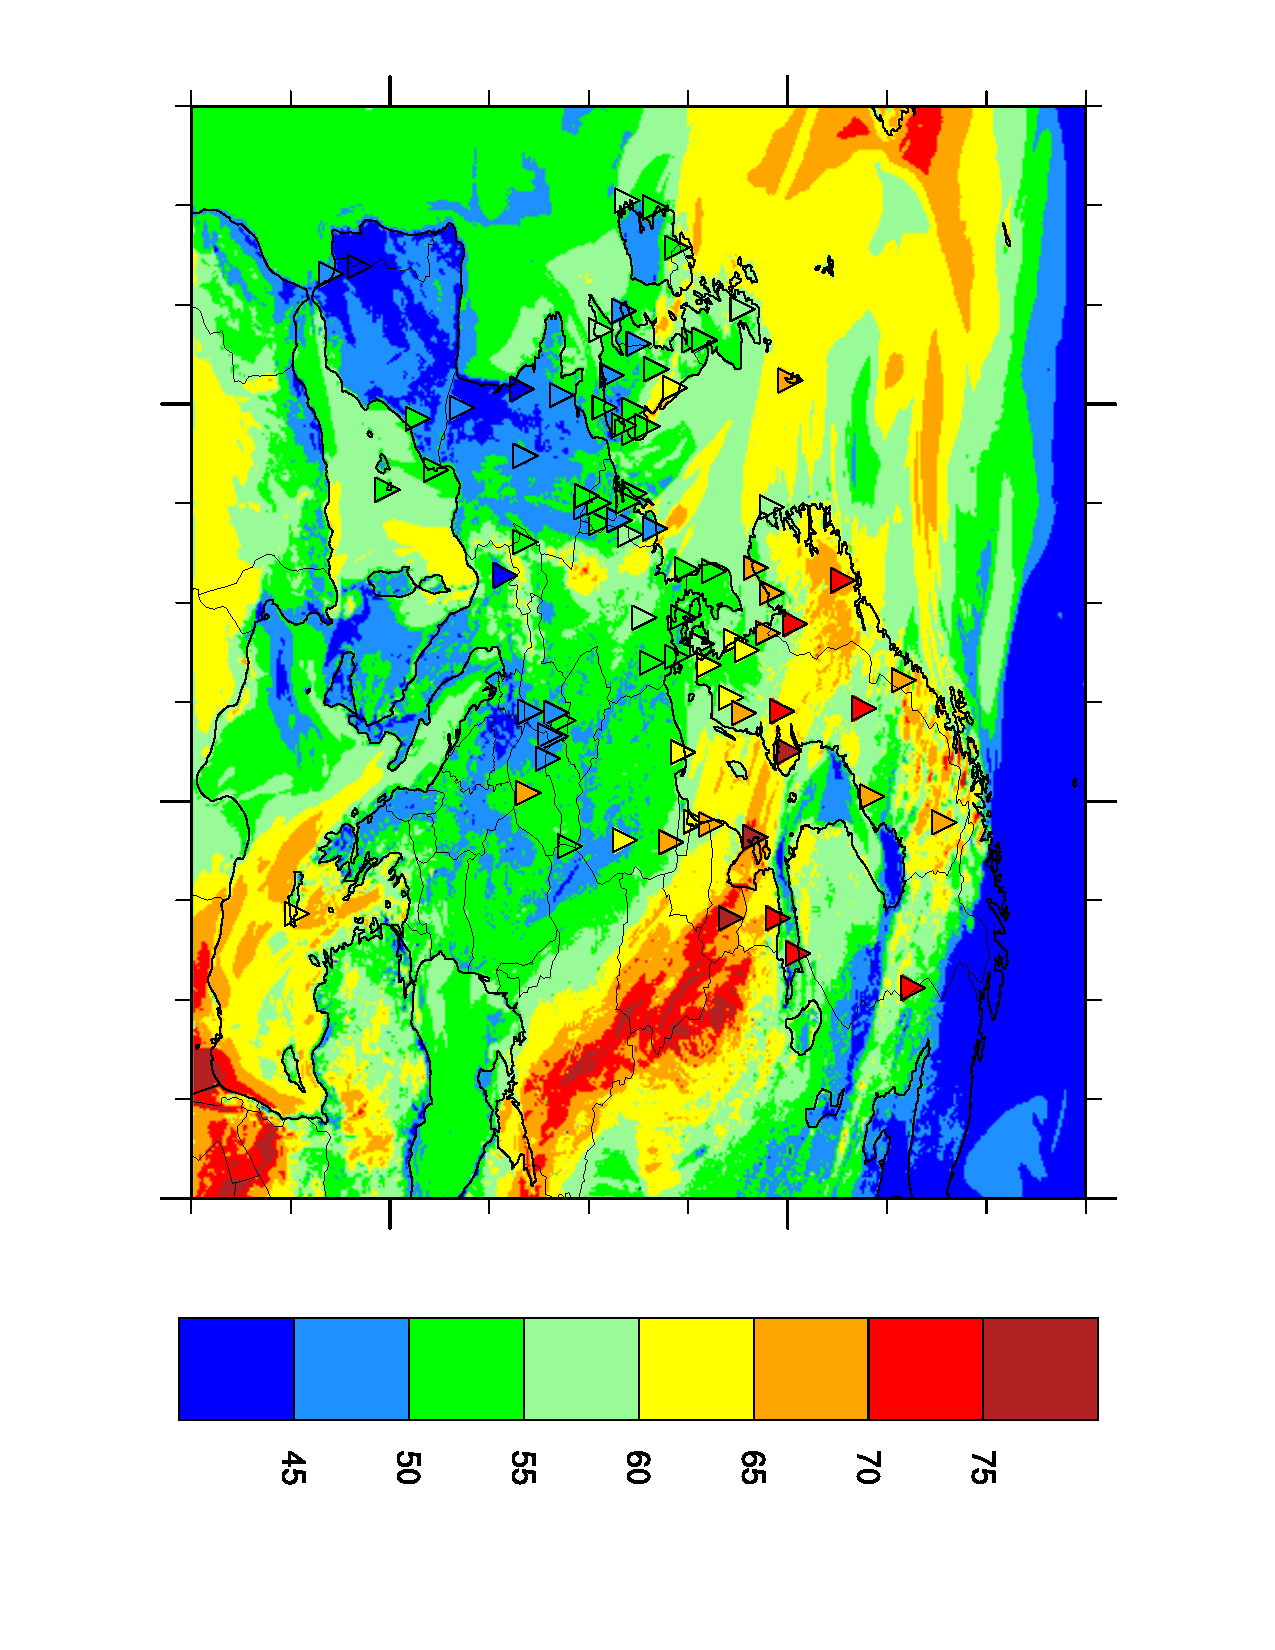
\includegraphics[clip=,angle=90,height=7.5cm,viewport=105 58 510 775]{FIGS_O3/20190424_MAXO3_ModObs_emep_H500.pdf}}
\caption{Modelled and measured daily max ozone [ppb] 24 April 2019.}
\label{fig:O3_20190424}
\end{figure}

June 2019 was the warmest June on record, globally as well as for Europe (\citep{Bissolli:2020}). During 26-28 June a persistent high pressure over central Europe brought very hot air masses into central and western parts of the continent. In Germany, temperatures just below 40 \degrees C was observed and in France 13 stations surpassed France’s 2003 records, exceeding a temperature of 44.1 \degrees C. Surface ozone levels above EU's information threshold (180 \ug) were observed in many countries during this period. At Ispra in Italy an extreme level of 142 ppb (285 \ug) was reported on 28 June, breaking EU's alert threshold of 240 \ug. Figure~\ref{fig:O3_20190628} shows the modelled and observed daily maximum ozone levels for 28 June. 

\begin{figure}[H]
  \centering{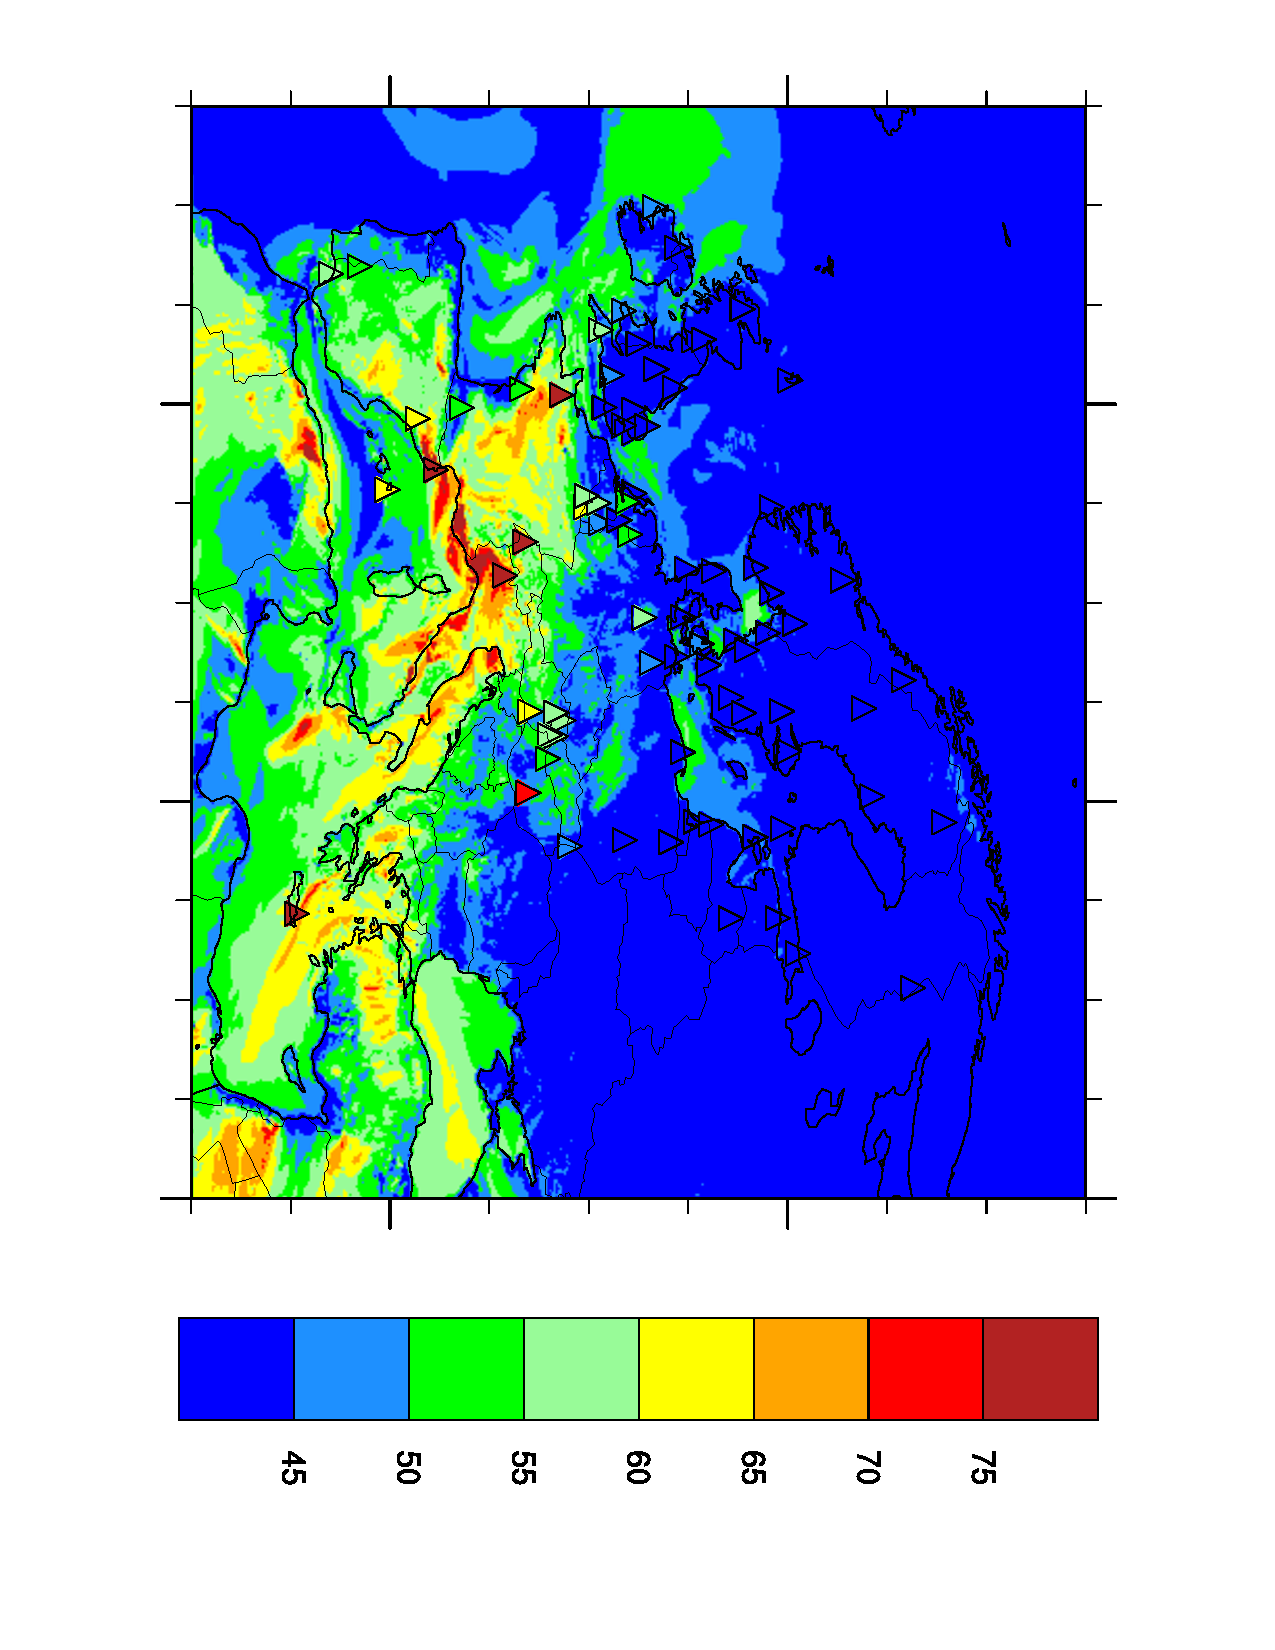
\includegraphics[clip=,angle=90,height=7.5cm,viewport=105 58 510 775]{FIGS_O3/20190628_MAXO3_ModObs_emep_H500.pdf}}
\caption{Modelled and measured daily max ozone [ppb] 28 June 2019.}
\label{fig:O3_20190628}
\end{figure}

One month later, during 24-26 July a new and even more intense (albeit shorter) heat wave struck central and northwestern part of Europe, and national temperature records were set in the UK and Germany (38.7 \degrees C in the UK and 40.5 \degrees C in Germany). Along with this heat wave, peak ozone levels were measured. In the UK, an hourly maximum level of 119 ppb (238 \ug) was observed at Sibton 25 July, the highest level measured at this site since 1996. At Vredepeel in the Netherlands, the ozone levels peaked at 127 ppb (254 \ug) on the same day and thereby broke EU's alert threshold. The extent of the ozone episode on 25 July is seen on Figure~\ref{fig:O3_20190725}, showing the modelled and observed values. 

\begin{figure}[H]
  \centering{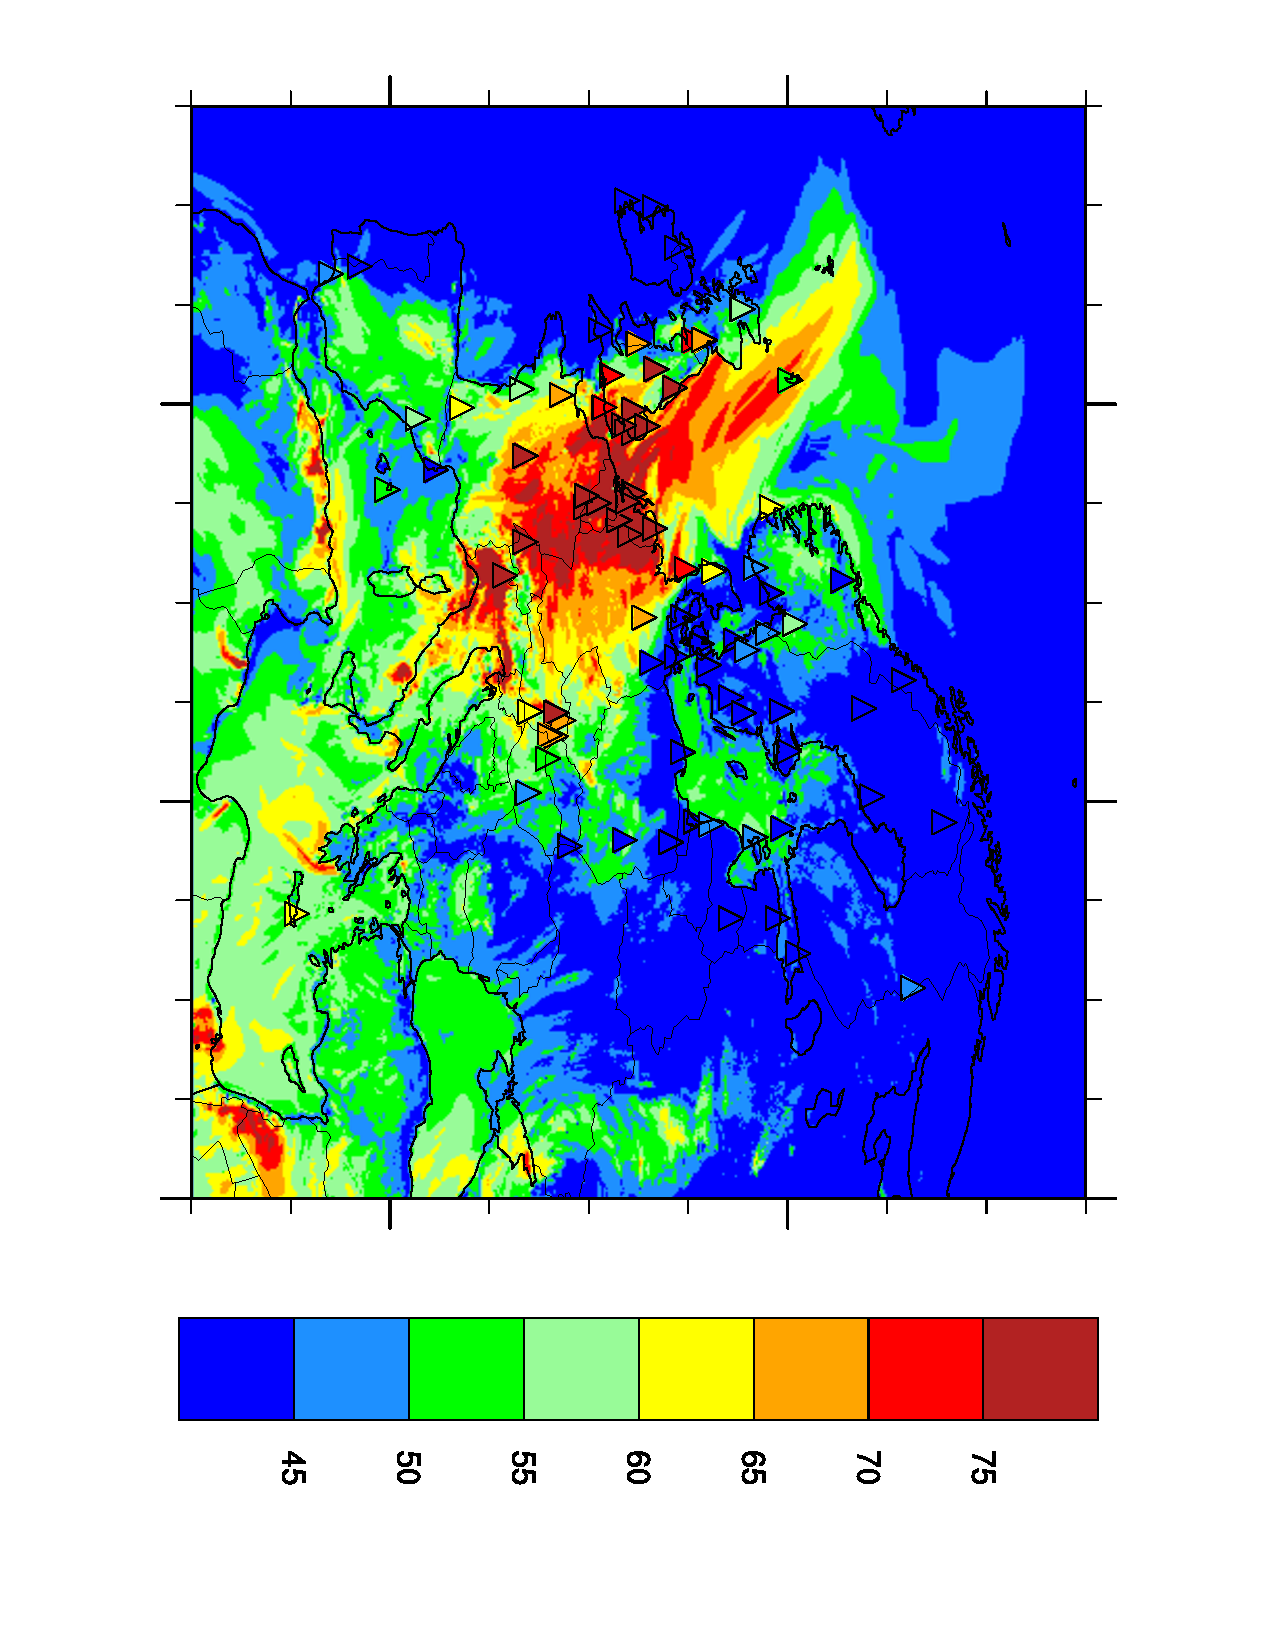
\includegraphics[clip=,angle=90,height=7.5cm,viewport=105 58 510 775]{FIGS_O3/20190725_MAXO3_ModObs_emep_H500.pdf}}
\caption{Modelled and measured daily max ozone [ppb] 25 July 2019.}
\label{fig:O3_20190725}
\end{figure}

For the year 2019 as a whole, Figure~\ref{fig:indicators_emep} shows various modelled ozone metrics with the corresponding measured metrics based on the EMEP measurement sites plotted on top of the maps. Only stations located below 500 metres above sea level were used in this comparison to avoid uncertainties related to the extraction of model data in regions with complex topography. Figure ~\ref{fig:indicators_emep} shows a) maxO3 (= mean of the daily max ozone concentration) for the 6-month period April-September, b) SOMO35 (= Sum of Ozone Means Over 35 ppb), c) AOT40 for forests (= Accumulated Ozone exposure over a Threshold of 40 ppb) for the 6-month period April-September using the hours between 08 and 20, and Figure~\ref{fig:indicatorPOD} shows POD$_1$ for forests (= Phytotoxic Ozone Dose above a threshold 1 mmol m$^{-2}$). Figure~\ref{fig:indicatorPOD} shows only modelled POD$_1$ since measurements could not be calculated from the ozone monitoring data directly and could not be included.

\begin{figure}[H]
  \centering
  \subfigure[maxO3]{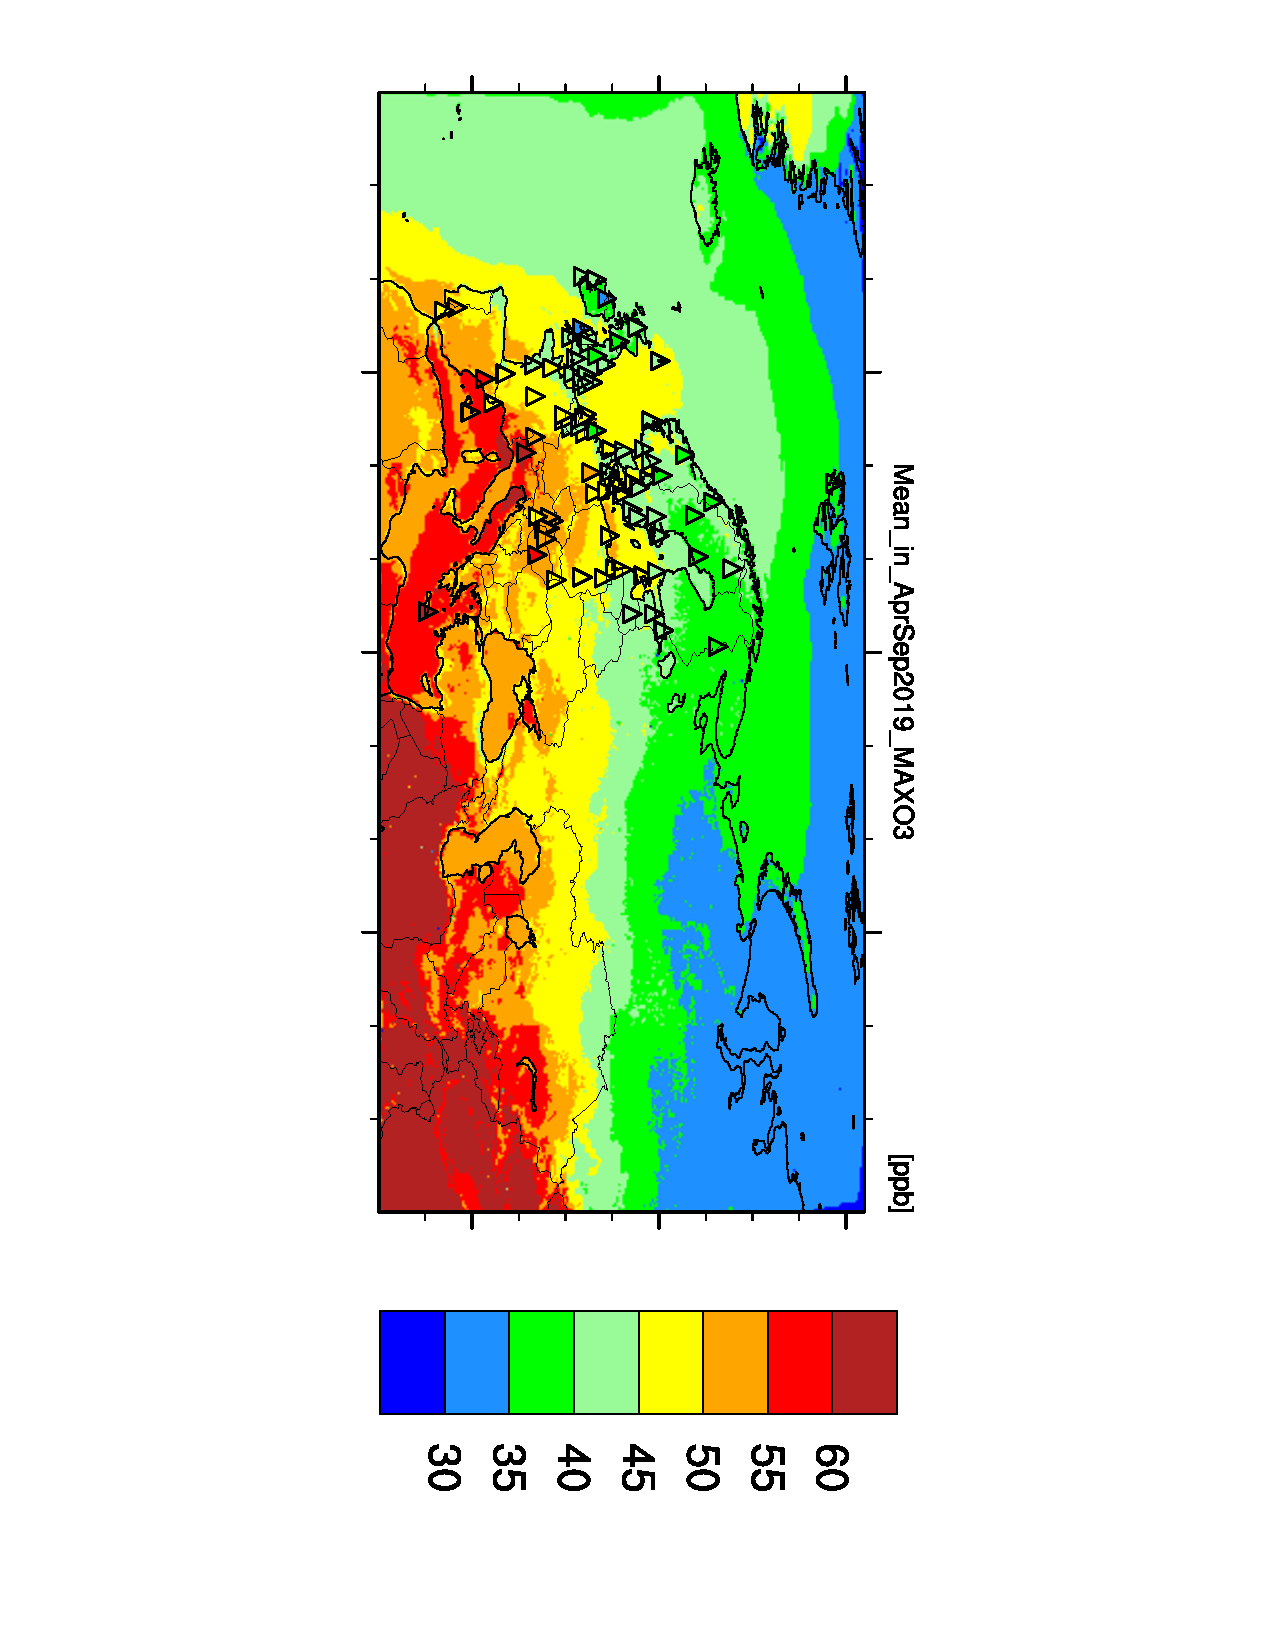
\includegraphics[clip=,angle=90,height=5.5cm,viewport=175 58 420 770]{FIGS_STATUS/MAXO3_AprSep_ModObs_emep_EMEP01.pdf}}
  \subfigure[SOMO35]{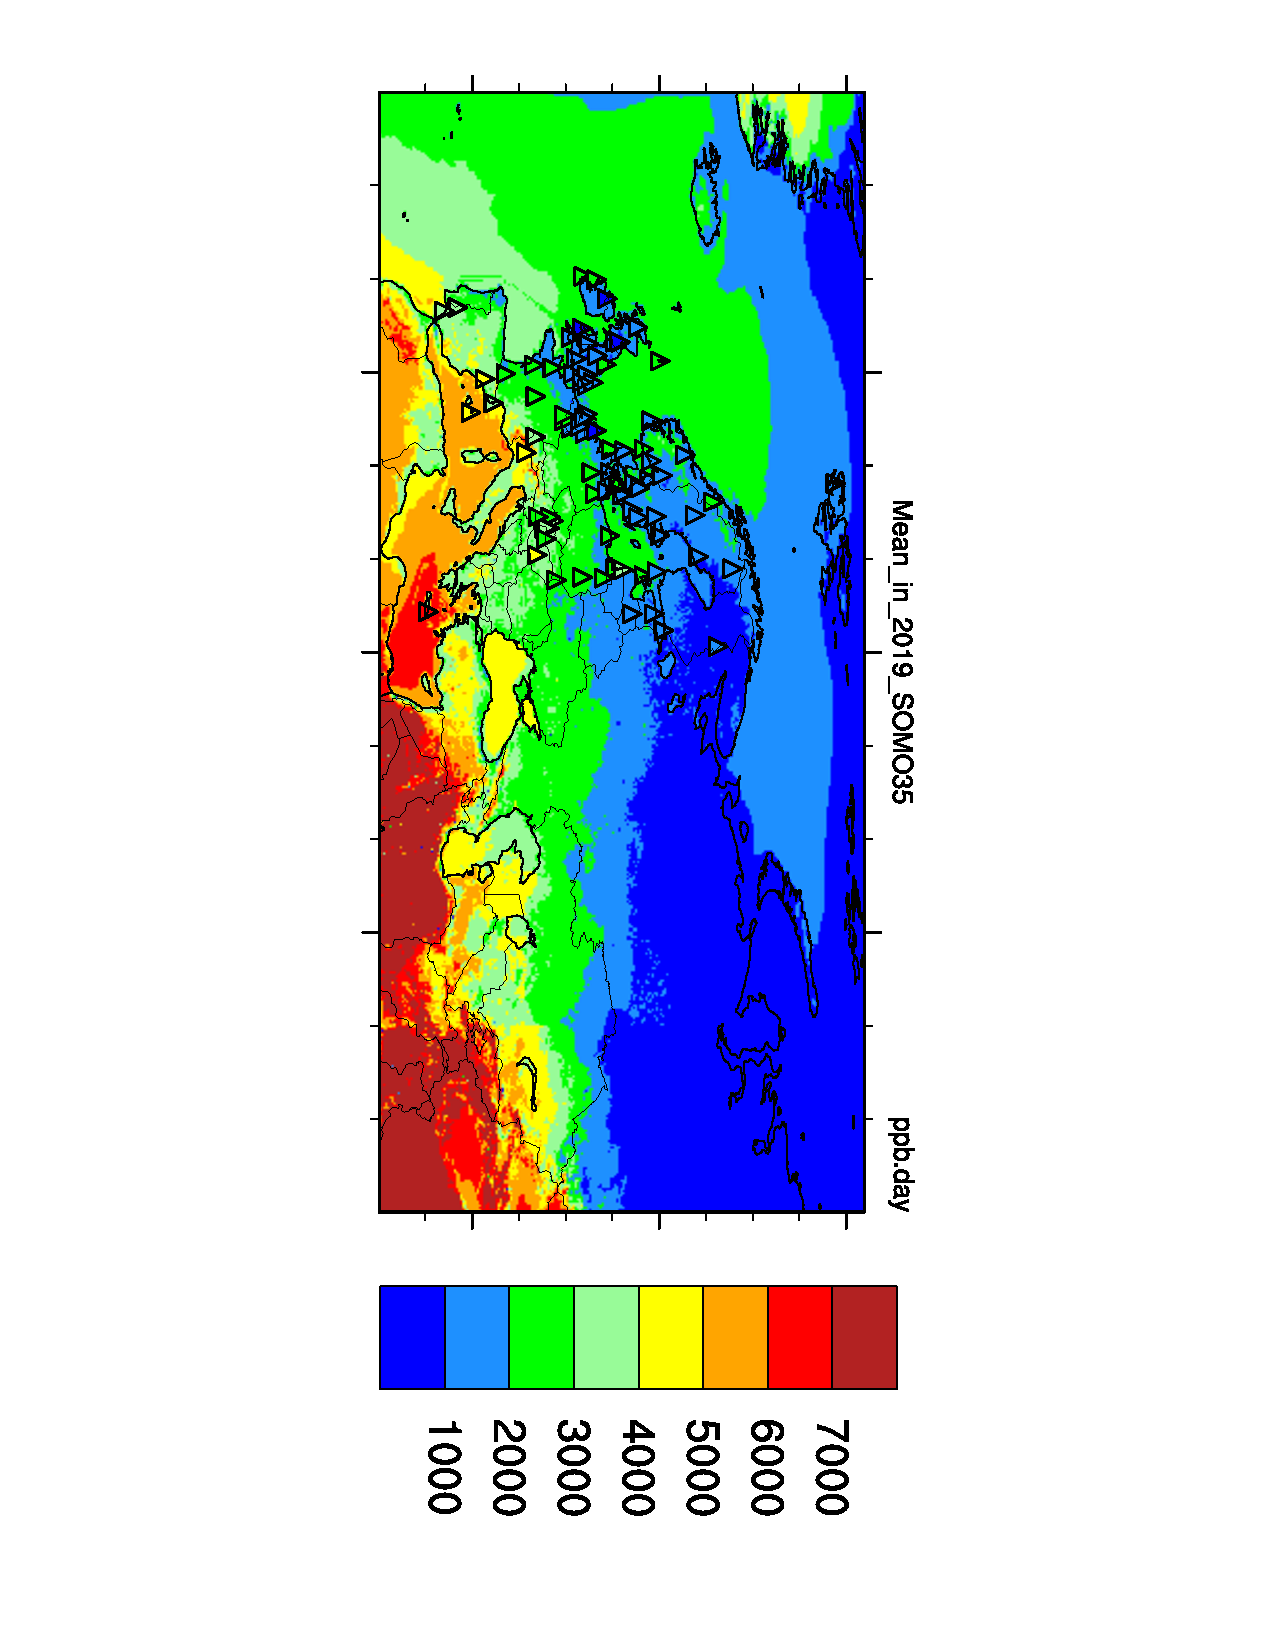
\includegraphics[clip=,angle=90,height=5.5cm,viewport=175 58 420 770]{FIGS_STATUS/SOMO35_ModObs_emep_EMEP01_L20EC.pdf}}
  \subfigure[AOT40]{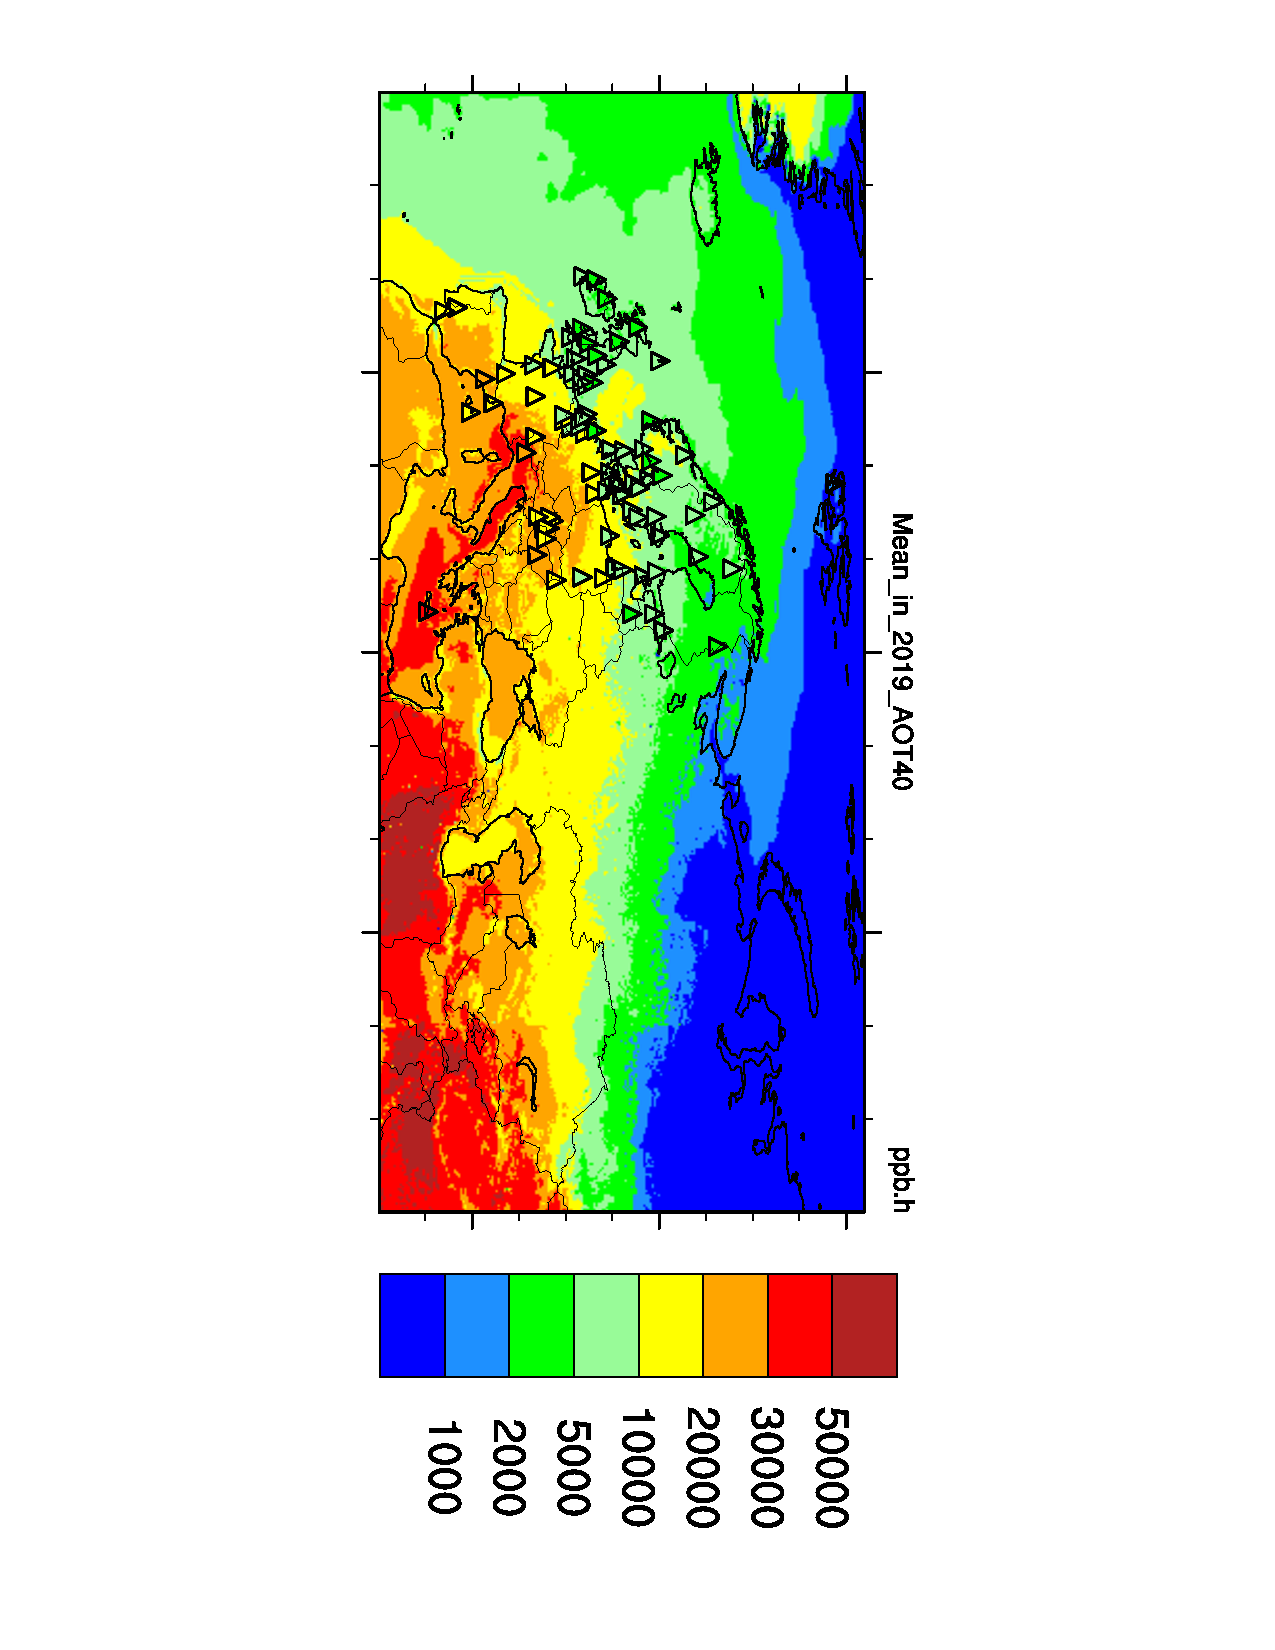
\includegraphics[clip=,angle=90,height=5.5cm,viewport=175 58 420 770]{FIGS_STATUS/AOT40_ModObs_emep_EMEP01_L20EC.pdf}}
\caption{Model results and observations at EMEP stations (triangles) for mean of daily maximum ozone concentrations (a) ([$ppb$], Apr-Sep), SOMO35 (b) [$ppb.d$] and AOT40 for forests (c) [$ppb.h$] in 2019. Only data from measurement sites below 500 m a.s.l. are shown.}
\label{fig:indicators_emep}
\end{figure}


These plots indicate good agreement between these modelled and measured ozone metrics in general. The model and the measurements show an increasing gradient to the southeast as expected which reflects the strong dependency between surface ozone, temperature and solar radiation. 

\begin{figure}[H]
  \centering{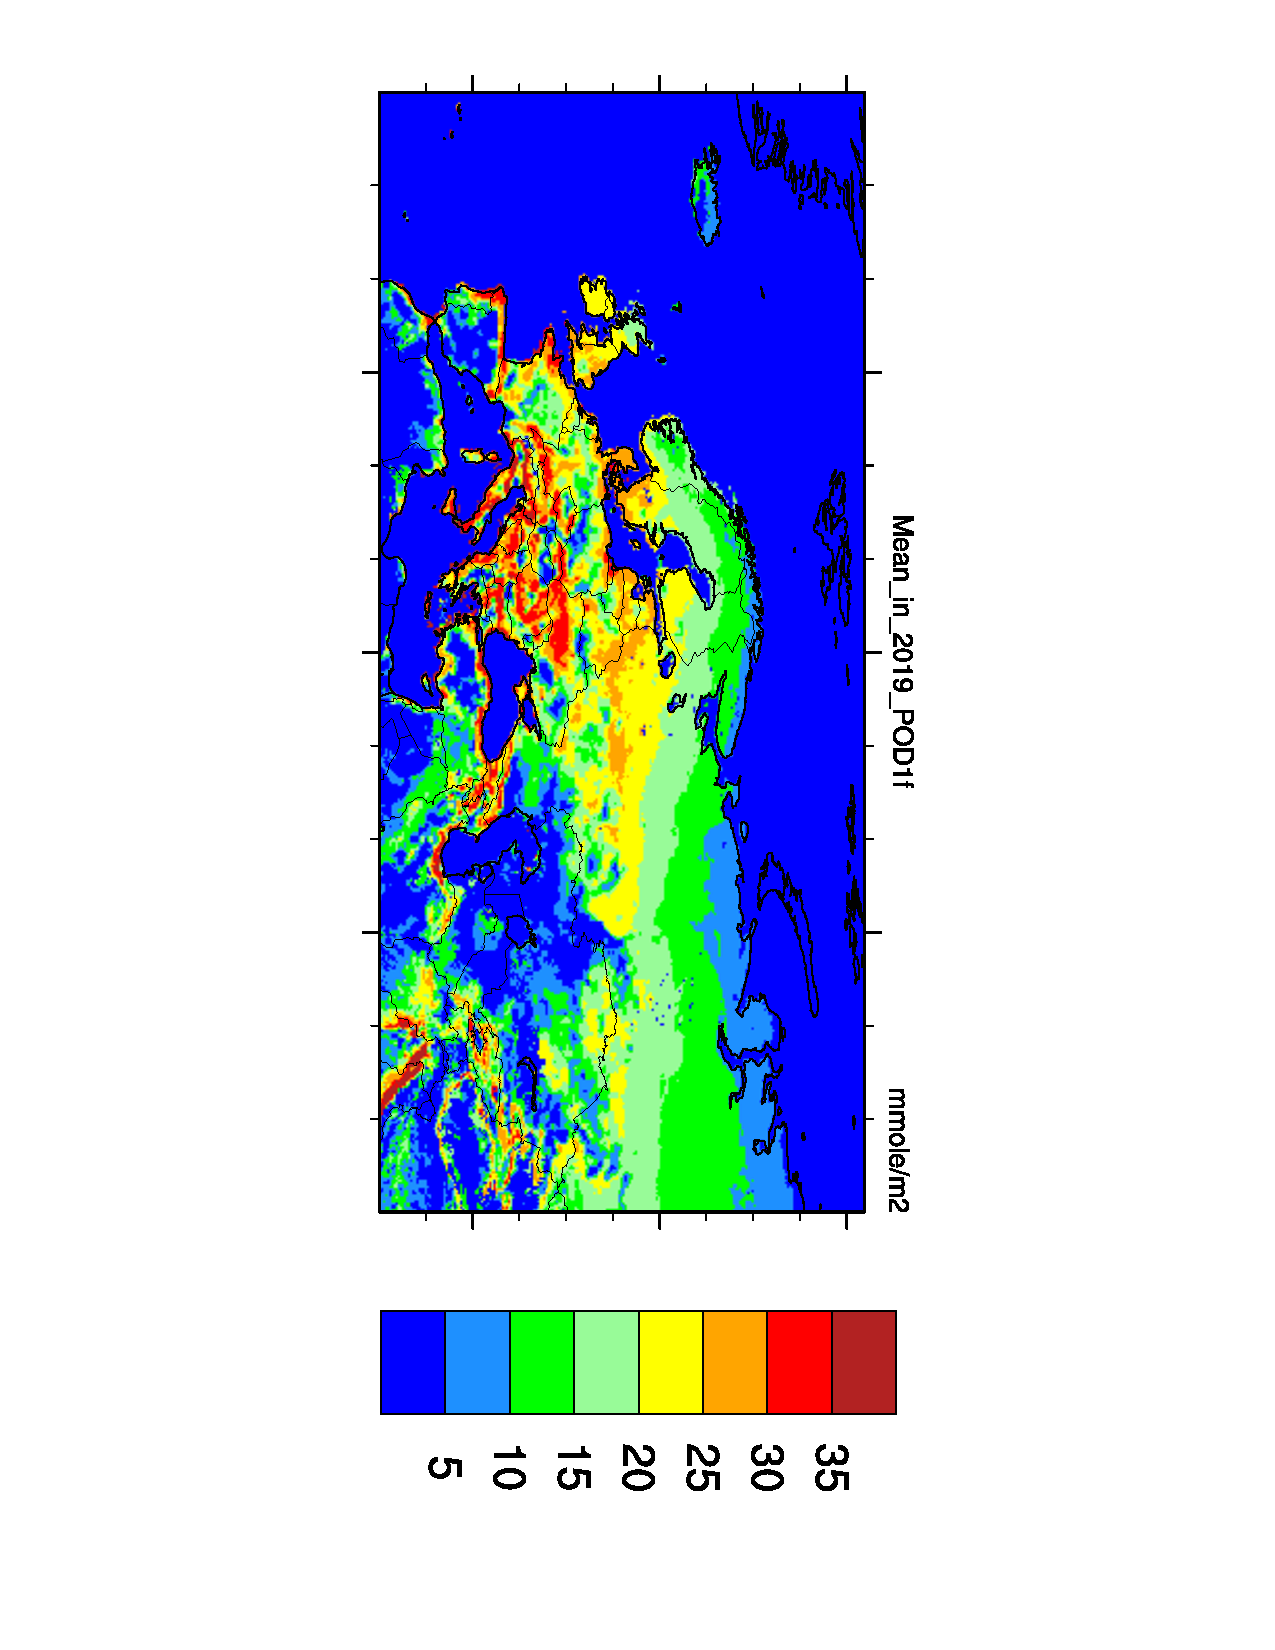
\includegraphics[clip=,angle=90,height=5.5cm,viewport=175 58 420 770]{FIGS_STATUS/POD1f_ModObs_emep_EMEP01.pdf}}
\caption{Model results of POD$_1$ for forests [$mmol m^-2$] in 2019}
\label{fig:indicatorPOD}
\end{figure}

It should be noted that the O$_3$ metrics such as AOT40 are very sensitive to the calculation of vertical O$_3$ gradients between the middle of the surface layer and the 3m height used for comparison with measurements \citep{Tuovinen:EP2007} and thus more difficult to compare with measurement data than, e.g., the mean daily maximum. Indeed, the formulation we use \citep{Simpson:EMEP2012} is probably better suited to a lowest model layer of 90m thickness (since we equate the centre of this, ca. 45m, with a `blending-height') than to a lowest model layer of 50m thickness (as used throughout this report). 
The modelled POD$_1$ pattern differs from the other metrics reflecting the influence of additional parameters such as plant physiology, soil moisture etc., and is a metric more indicative of the direct impact of ozone on vegetation than, e.g., AOT40. The POD$_1$ field could, however, not be validated by the EMEP ozone measurement data alone. 

SOMO35 is an indicator for health impacts recommended by WHO, and the results given in Figure~\ref{fig:indicators_emep} indicate that the health risk associated with surface ozone increased towards southern Europe. Highest levels are seen in the Mediterranean area and Northern Italy. SOMO35 is a health risk indicator without any specific threshold or limit value.

AOT40 and POD$_1$ are indicators for effects on vegetation. UNECE's critical level for forests based on the 6-months AOT40 value is 5000 ppb hours, and the results shown in Figure~\ref{fig:indicators_emep} indicate that this level was exceeded in most of Europe in 2019 although the model tends to overestimate the AOT40 values somewhat. In parts of central and south Europe the critical level was exceeded by a very large margin (20000 ppb hours and more). During dry periods, plants will reduce or close their stomata as a response to soil water deficit, which in turn will lead to reduced uptake of ozone.  Parts of the reason for the elevated atmospheric concentrations of ozone (and the high AOT40 levels) could thus be explained by the reduced uptake in vegetation.

On the contrary, POD$_1$ takes into account this soil moisture deficit, giving an estimate of the actual flux of ozone into the plants. It is interesting to see the substantial difference in the geographical pattern of AOT40 and POD$_1$ in Figures~\ref{fig:indicators_emep} (c) and \ref{fig:indicatorPOD}. Whereas AOT40 shows a north-south gradient with peak values over southern/central parts of the continent, POD$_1$ is highest along the coast and shows a minimum in central parts of Europe just where high values of AOT40 are seen. This reflects the importance of the soil moisture effect for these two metrics for ozone damage to vegetation. For POD$_1$ the limit value depends on the species and Mills et al (2011) give a value of 4 mmol m$^{-2}$ for birch and beech and 8 mmol m$^{-2}$ for Norway spruce. The results in Figures~\ref{fig:indicators_emep} (c) and \ref{fig:indicatorPOD} indicate that both these limit values were exceeded in most of Europe. The modelled levels of POD$_1$ could, however, not be validated by observations. 

Surface ozone levels and the associated metrics were fairly high in 2019 which partly could be explained by several heat waves striking the continent in the summer half year. This is an indication of the strong link between climate and surface ozone and raises the issue of climate induced changes of ozone in the years to come. A main question is to what extent such changes will outweigh the benefits of reduced ozone precursors emissions. 


%=========================================
\subsection{Particulate matter} 
\label{subs:PMstatus}

Maps of annual mean concentrations of \PM[10] and \PM[2.5] in 2019,
calculated by the EMEP MSC-W model, are presented in
Figure~\ref{fig:PMin2019}. The figures also show annual mean \PM[10]
and \PM[2.5] concentrations observed at the EMEP monitoring network,
which are represented by colour triangles overlaying the contours of the
modelled concentration fields.

\begin{figure}[H]
  \centering{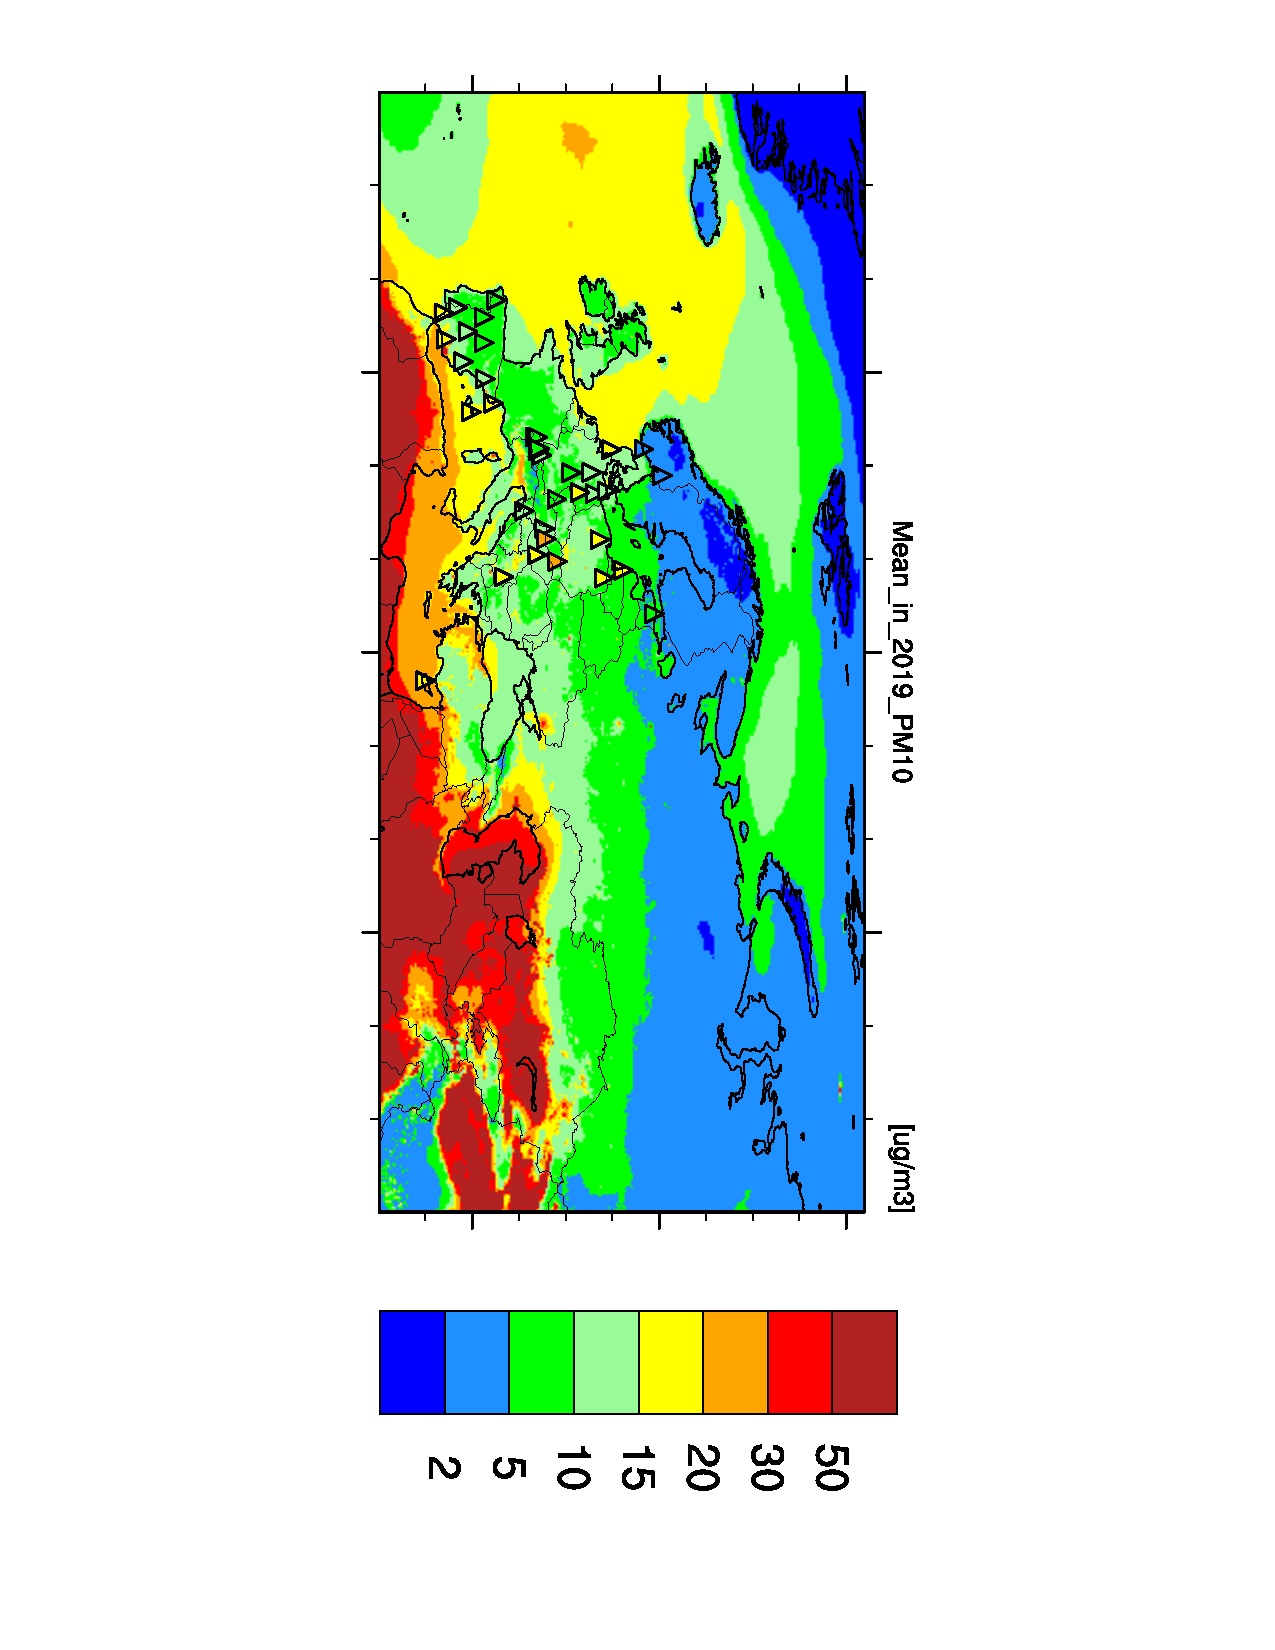
\includegraphics[clip=,angle=90,height=6cm,viewport=175 67 448 754]{FIGS_PM/Mean_in_2019_PM10_EMEP01_ALL.pdf}}\\
  \vspace{0.5cm}
  \centering{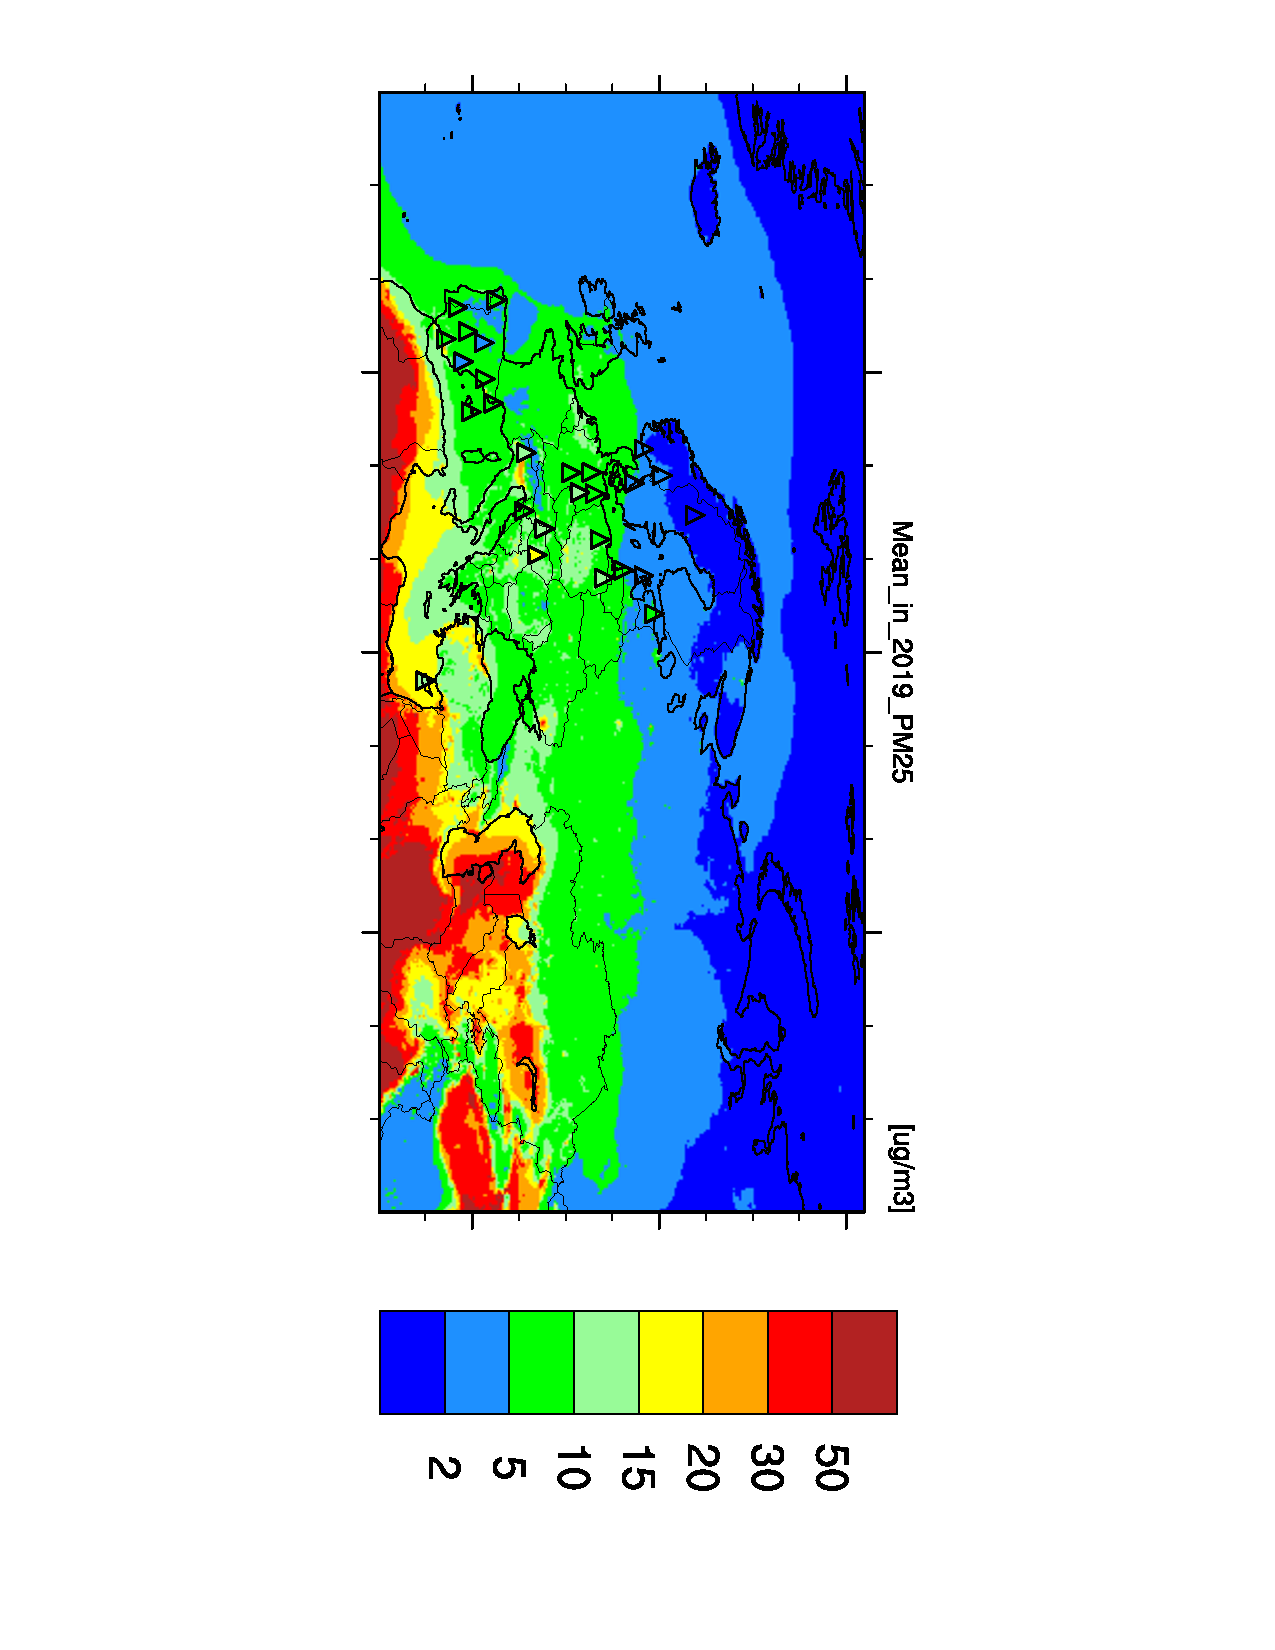
\includegraphics[clip=,angle=90,height=6cm,viewport=175 67 448 754]{FIGS_PM/Mean_in_2019_PM25_EMEP01_ALL.pdf}}
\caption{Annual mean concentrations of \PM[10] and \PM[2.5] in 2019:
  calculated with the EMEP MSC-W model (colour contours) and observed
  at EMEP monitoring network sites (colour triangles). \textit{Note:
    Observations include hourly, daily and weekly data.}}
\label{fig:PMin2019}
\end{figure}


The model results and the observations are well in agreement
regarding the geographical distribution of the annual mean levels of
\PM[10] and \PM[2.5], showing their general increase over land from
north to south. The concentrations are below 2-5 \ug in Northern
Europe, increasing to 5-15 \ug in the mid-latitudes and further south,
\PM[2.5] levels being somewhat lower than those of
\PM[10]. Figure~\ref{fig:PMin2019} displays fairly homogeneous modelled levels of regional background PM over most of Central and Western Europe,
with \PM[10] in excess of 20 \ug in the Po Valley and on Cyprus. The observations also show \PM[10] concentrations above 20 \ug in Slovakia. \PM[2.5] concentrations are below 10 \ug over most of EMEP domain (except the south/southeast most regions), or otherwise between 10 and 15 \ug in  parts of Benelux, Poland, Hungary and some of Balkan countries). The only site with observed annual mean \PM[10] above 15 \ug (namely 16.3 \ug) was Hungarian K-Puszta. Furthermore, the model calculates high PM for the regions east of the Caspian Sea (parts of Kazakhstan, Uzbekistan, Turkmenistan) and over the southern Mediterranean, with annual mean concentrations in excess of 50 \ug. These high PM concentrations are due to windblown dust from the arid soils and deserts of Central Asia, though the accurateness of the calculated values still cannot be verified due to the lack of observations in these regions.

There is a good agreement between the modelled and observed
distributions of annual mean \PM[10] and \PM[2.5], with correlation
coefficients of 0.60 and 0.72, respectively. Overall, the model
underestimates the observed annual mean of \PM[10] by 12\% and
\PM[2.5] by 13\% (see also Table \ref{tab:tableOldFashioned} in \ref{ch:appx_modeleval}). \textcolor{blue}{CHECK with and Refer to AeroVal....}


Overall, the year of 2019 was quite moderate with respect to PM air pollution in Europe, which was due to dominating meteorological conditions that year. It was relatively warm across the EMEP area (Figure~\ref{fig:metyear-avMET}), in particular in the cold half-year (Figure~\ref{fig:temp-avMET}). Mild winter conditions would mean less need for residential heating, resulting in lower emissions from this sector. Moreover, stagnant air conditions (with temperature inversion, low wind speed and thin mixing layer), typically causing elevated pollution levels, are less frequent in warm winters. Also, the spring/summer period was relatively warm (except from Russia, Kazakhstan, Finland, most of Sweden, Spain and Portugal). During those months, the higher temperatures would enhance evaporation of semi-volatile inorganic and organic aerosols (SIA and SOA), though the more efficient oxidation contributes to secondary aerosol formation. Furthermore, the year 2019 was relatively dry over most of Europe (except in the south and parts of Scandinavia), in EECCA countries, and most of Russia (except from the northern regions), as shown in Figure~\ref{fig:metyear-avMET}. However, the amount of precipitation was also relatively large in the cold half-year in Denmark, France, the UK and parts of Germany (Figure~\ref{fig:prec-avMET}). As documented in ~\citet{CAMS2020}, the wet end of the year in western and southern Europe was the most prominent feature of precipitation in 2019, with 
November being particularly extreme, both in terms of the total rainfall amounts and the number of days with heavy rainfall. As wet scavenging is the main PM removal mechanism, this, combined with the mild winter temperatures, resulted in the lower levels of PM pollution in winter 2019 over most of Europe.   

\begin{figure}[H]
  \centering{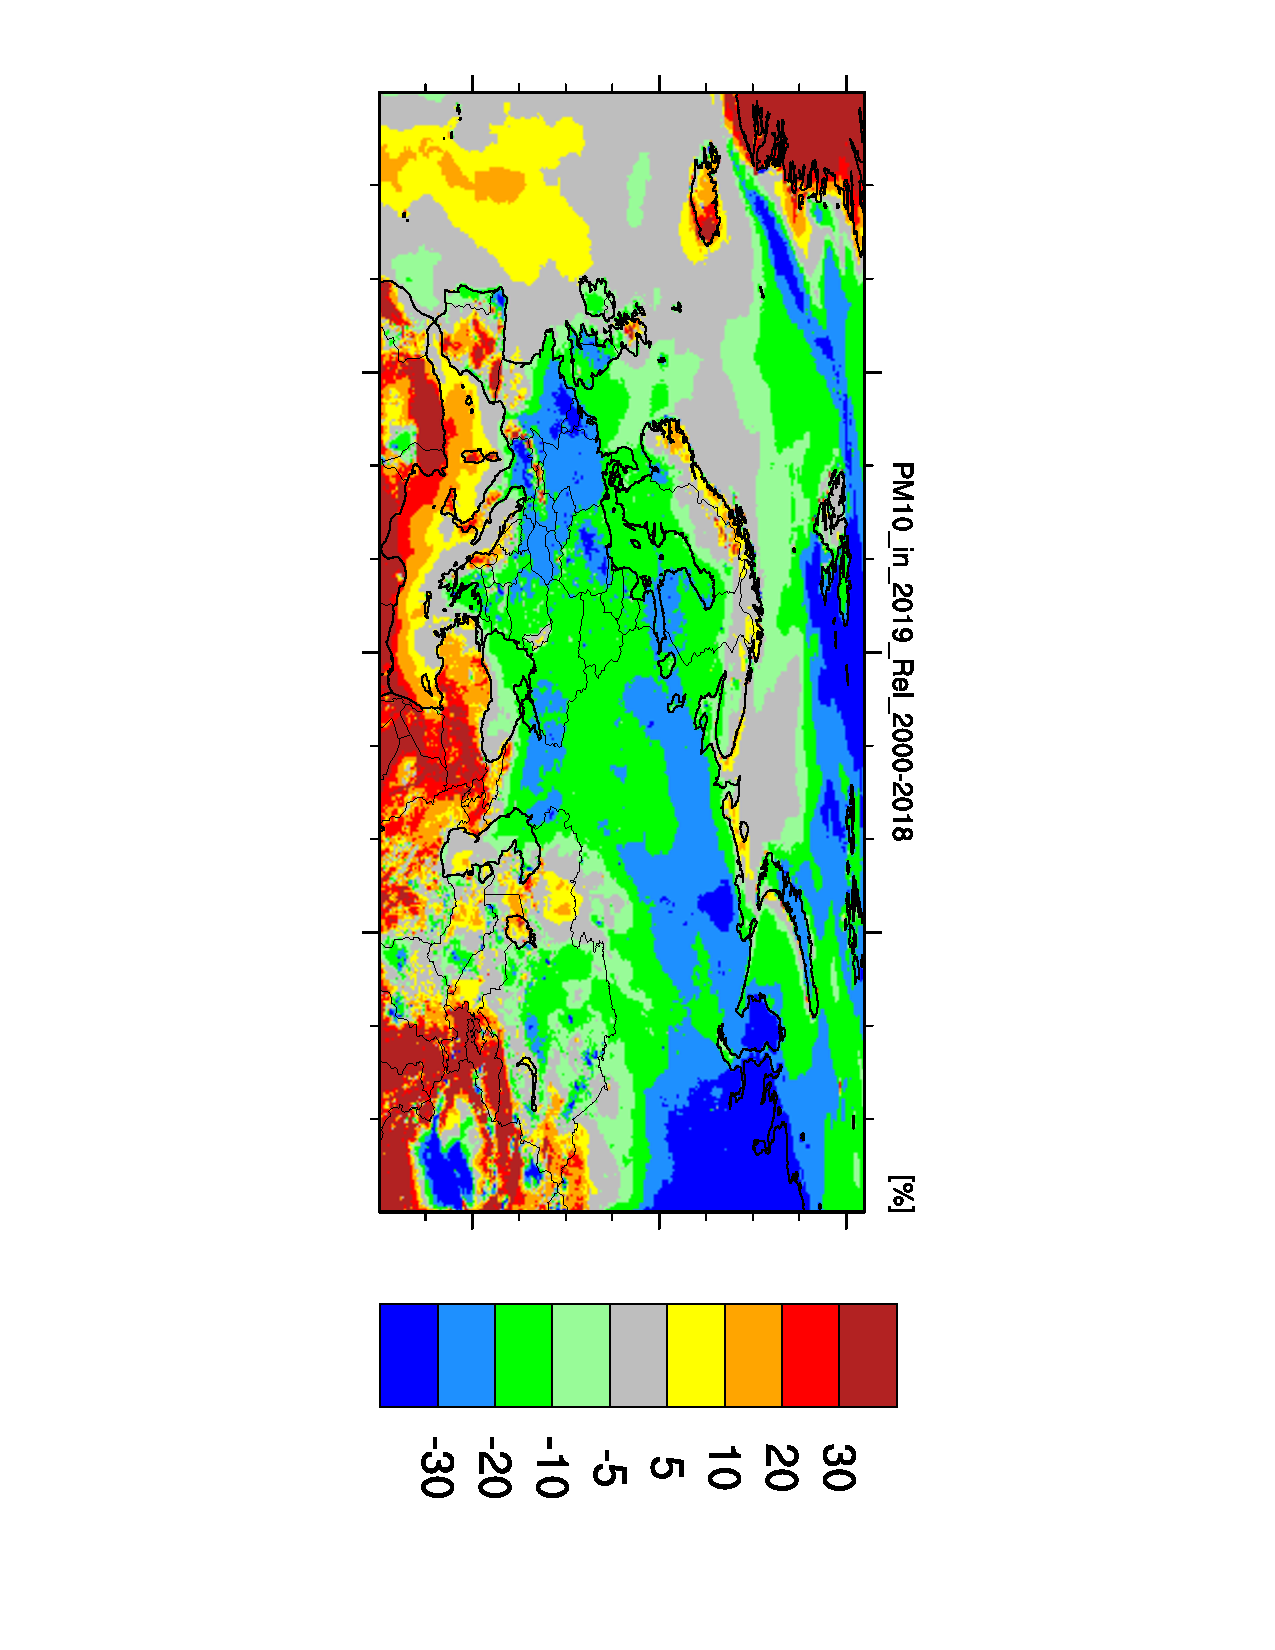
\includegraphics[clip=,angle=90,height=3cm,viewport=175 67 448 754]{FIGS_PM/RelAnomaly_PM10_2019_vs_2000-2018.pdf}}
  \centering{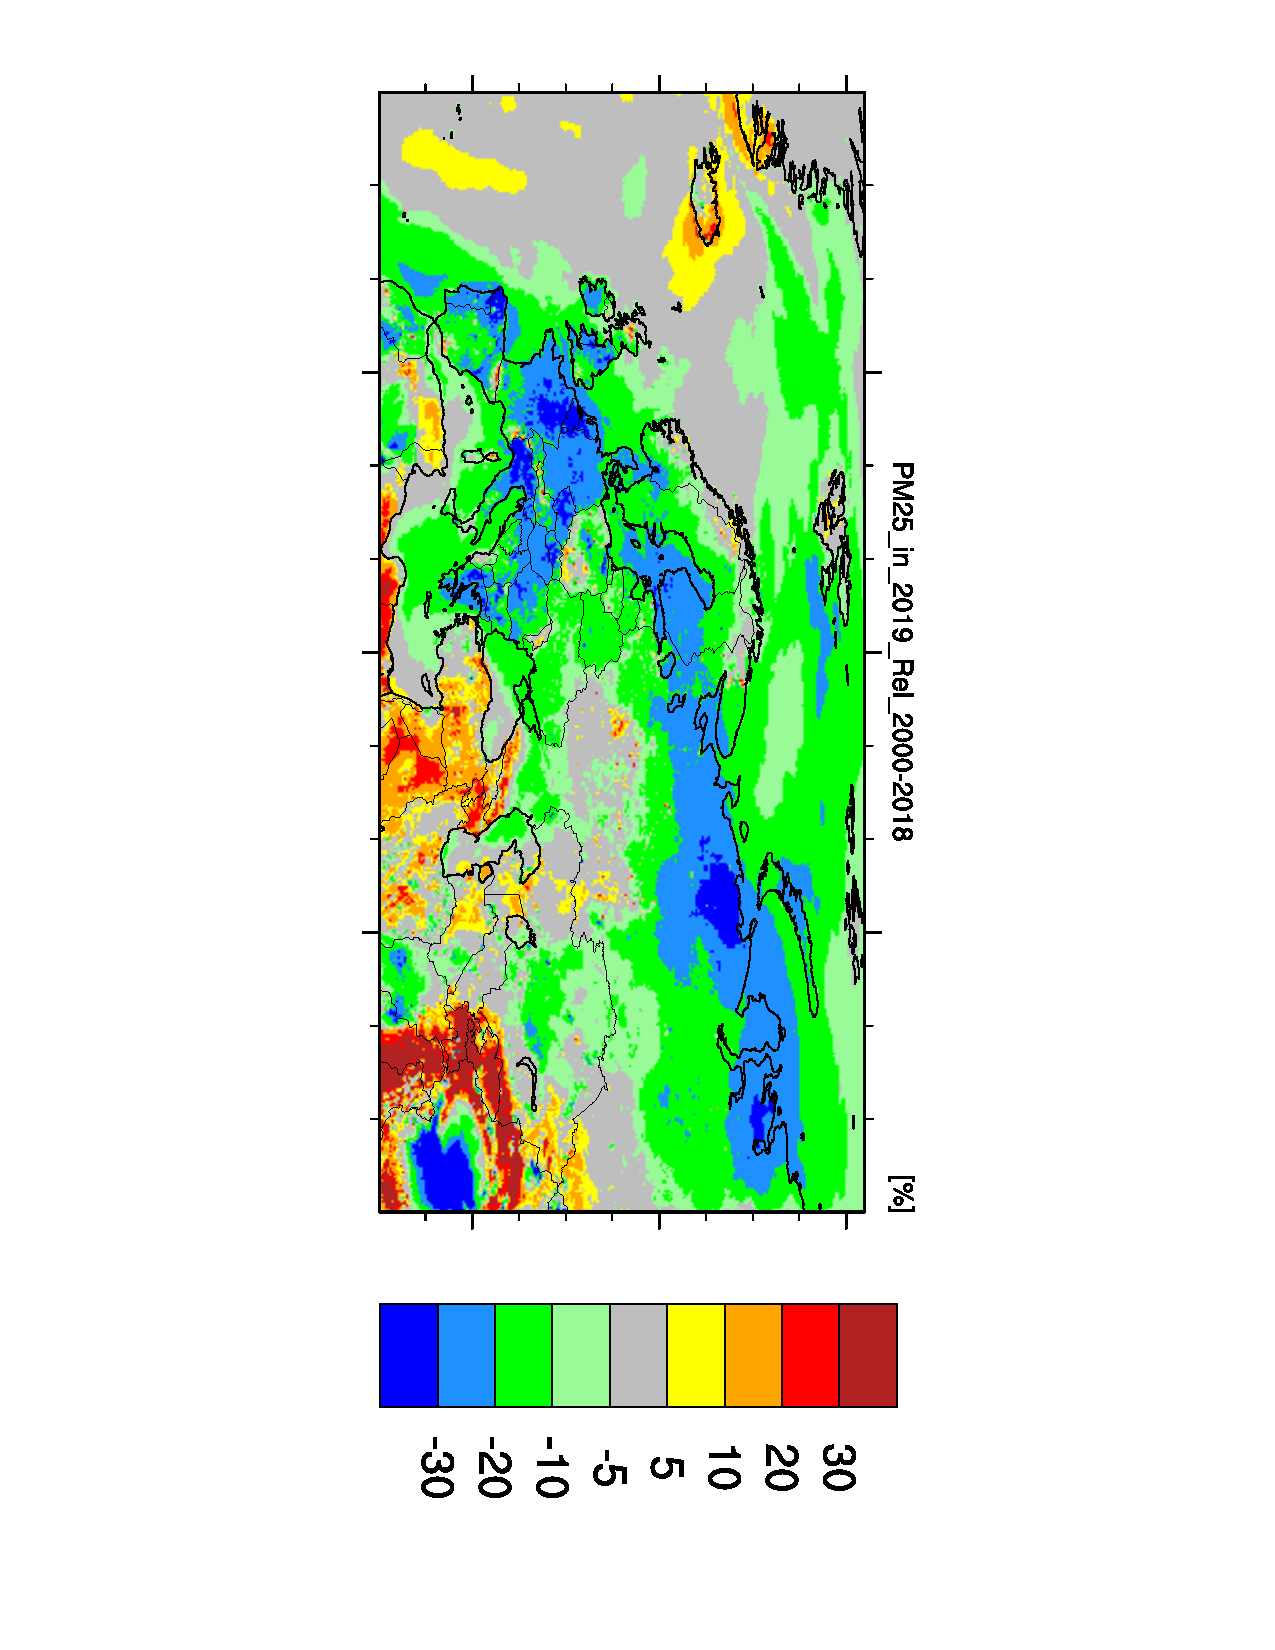
\includegraphics[clip=,angle=90,height=3cm,viewport=175 67 448 754]{FIGS_PM/RelAnomaly_PM25_2019_vs_2000-2018.pdf}}
\caption{Relative anomalies of mean \PM[10] and \PM[2.5] in 2019 from the 2000-2018 mean.}
\label{fig:PManomin2019}
\end{figure}

Figure~\ref{fig:PManomin2019} presents the relative anomalies of mean \PM[10] and \PM[2.5] concentrations in 2019 relative to 2000-2018 averages, based on the 2000-2019 trend runs performed with the EMEP MSC-W model using a consistent emission data-set based on officially submitted data, as documented in Chapter \ref{ch:Trends}. In order to look at the sole effect of meteorological conditions on PM pollution, also 2019 run used here is based on the reported emissions and thus different from the 2019 Status run (in which TNO's emissions for residential combustion are used, as documented in Section \ref{Mod_2019}). Figure~\ref{fig:PManomin2019} shows that the PM pollution in 2019 was relatively moderate, with annual mean concentrations being 5-20\% lower than the 2000-2018 averages over most of the EMEP domain, and 20-35\% lower compared to the 18-year average in Central Europe and over vast areas in the N/NE of Russia. Only along NW/N coasts in Fennoscandia, parts of Spain and some south-eastern regions (parts of Turkey, the Caucasus region and Central Asian countries), \PM[10] and \PM[2.5] levels in 2019 were higher relative to the 2000-2018 averages. 


\subsubsection[PM exceedances]{Exceedances of EU limit values and WHO Air Quality Guidelines in 2018}
\label{subsec:PMexc}

In this section we compare \PM[10] and \PM[2.5] exceedances
of EU critical limits and WHO recommended Air Quality
Guidelines \citep{WHO:AQG}, calculated by the EMEP MSC-W model, with
those measured at EMEP sites. The EU limit values for \PM[10] (Council
Directive 1999/30/EC) are 40 \ug for the annual mean and 50 \ug for
the daily mean concentrations, with the daily limit not to be exceeded
more than 35 times per calendar year~\citep{EU2008}. For \PM[2.5], the
annual mean limit value of 25 \ug entered into force on 01.01.2015.

The Air Quality Guidelines (AQG) recommended by WHO \citep{WHO:AQG}
are:
\begin{itemize}
\item for \PM[10]: 20 \ug annual mean, 50 \ug 24-hourly (99th perc. or 3 days per year)
\item for \PM[2.5]: 10 \ug annual mean, 25 \ug 24-hourly (99th perc. or 3 days per year)
\end{itemize}


The EU limit values for protection of human health from particulate
matter pollution and the WHO AQG for PM should apply to concentrations
for zones or agglomerations, in rural and urban areas,
which are representative for exposure of the general
population. \PM[10] and \PM[2.5] concentrations calculated with the
EMEP MSC-W model on the 0.1$\degrees \times$ 0.1$\degrees$ grid cannot
reproduce urban hotspot levels, but give a reasonable representation
of PM levels occurring in rural and, to some extend, in urban background
areas.


Model results and EMEP observational data show that the annual mean \PM[10] concentrations were below the EU limit value of 40 \ug for all of Europe in 2019 (Figure~\ref{fig:PMin2019}). The model calculates annual mean \PM[10] above the WHO recommended AQG of 20 \ug
in only small regions in the Po Valley and western Turkey. The highest
observed annual mean \PM[10] concentrations, exceeding the AQG of 20 \ug, were registered at Slovakian sites (24 \ug at SK0004 and 23 \ug SK0007) and Greek GR0001 (23 \ug, 58\% data coverage only). Further, the observations and model results show that annual mean \PM[2.5] concentrations (Figure~\ref{fig:PMin2019}) in 2019 were below the EU limit value of 25 \ug (except in the Po Valley according to the model). However, there were observed cases of exceedance of the WHO AQG value of 10 \ug by annual mean \PM[2.5] at nine sites (including GR0001 with 57\% data coverage), with the highest values at the Hungarian site HU0004 with 16 \ug, followed by German DE0044 with 14 \ug and Italian IT0004 with 13 \ug.


\begin{figure}[ht]
  \centering{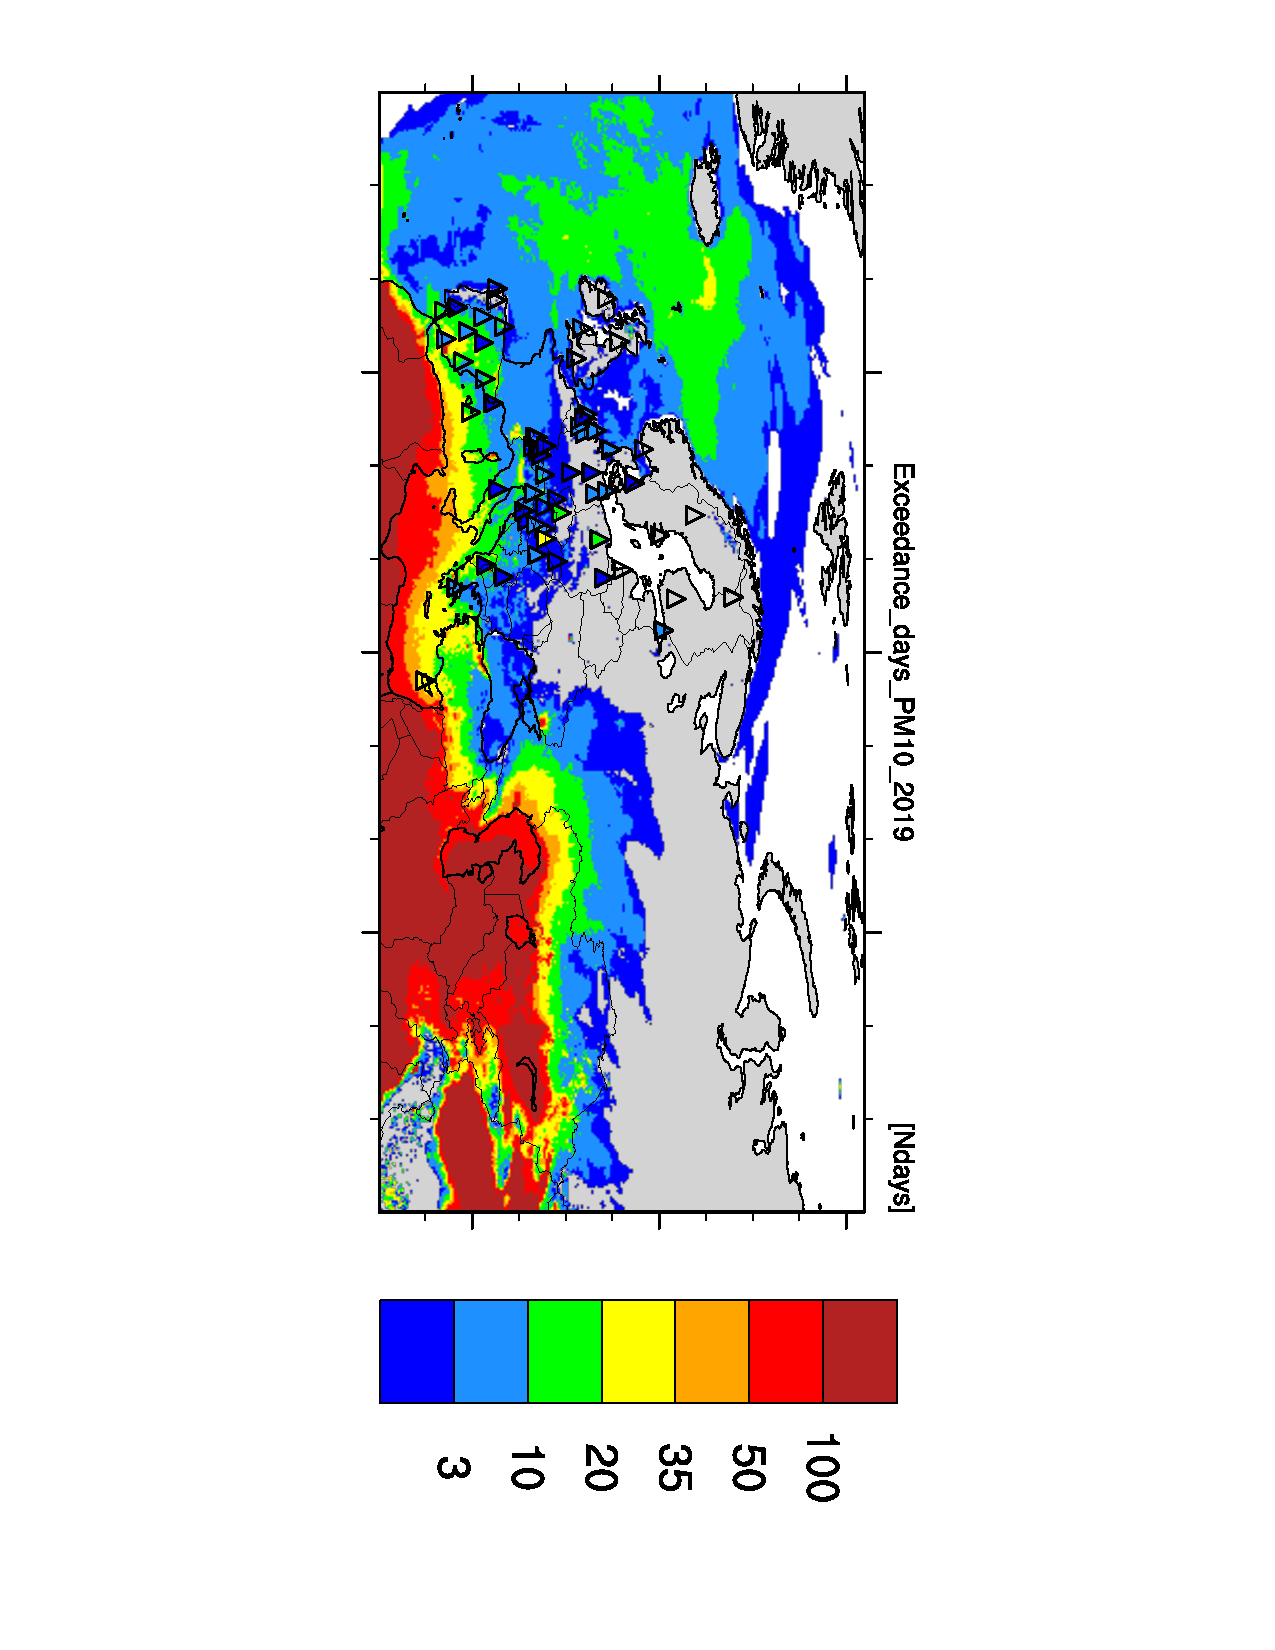
\includegraphics[clip=,angle=90,height=5.9cm,viewport=180 67 440 754]{FIGS_PM/ExcDays_PM10_ModObs_EMEP01_2019.pdf}}\\
  \vspace{0.5cm}
  \centering{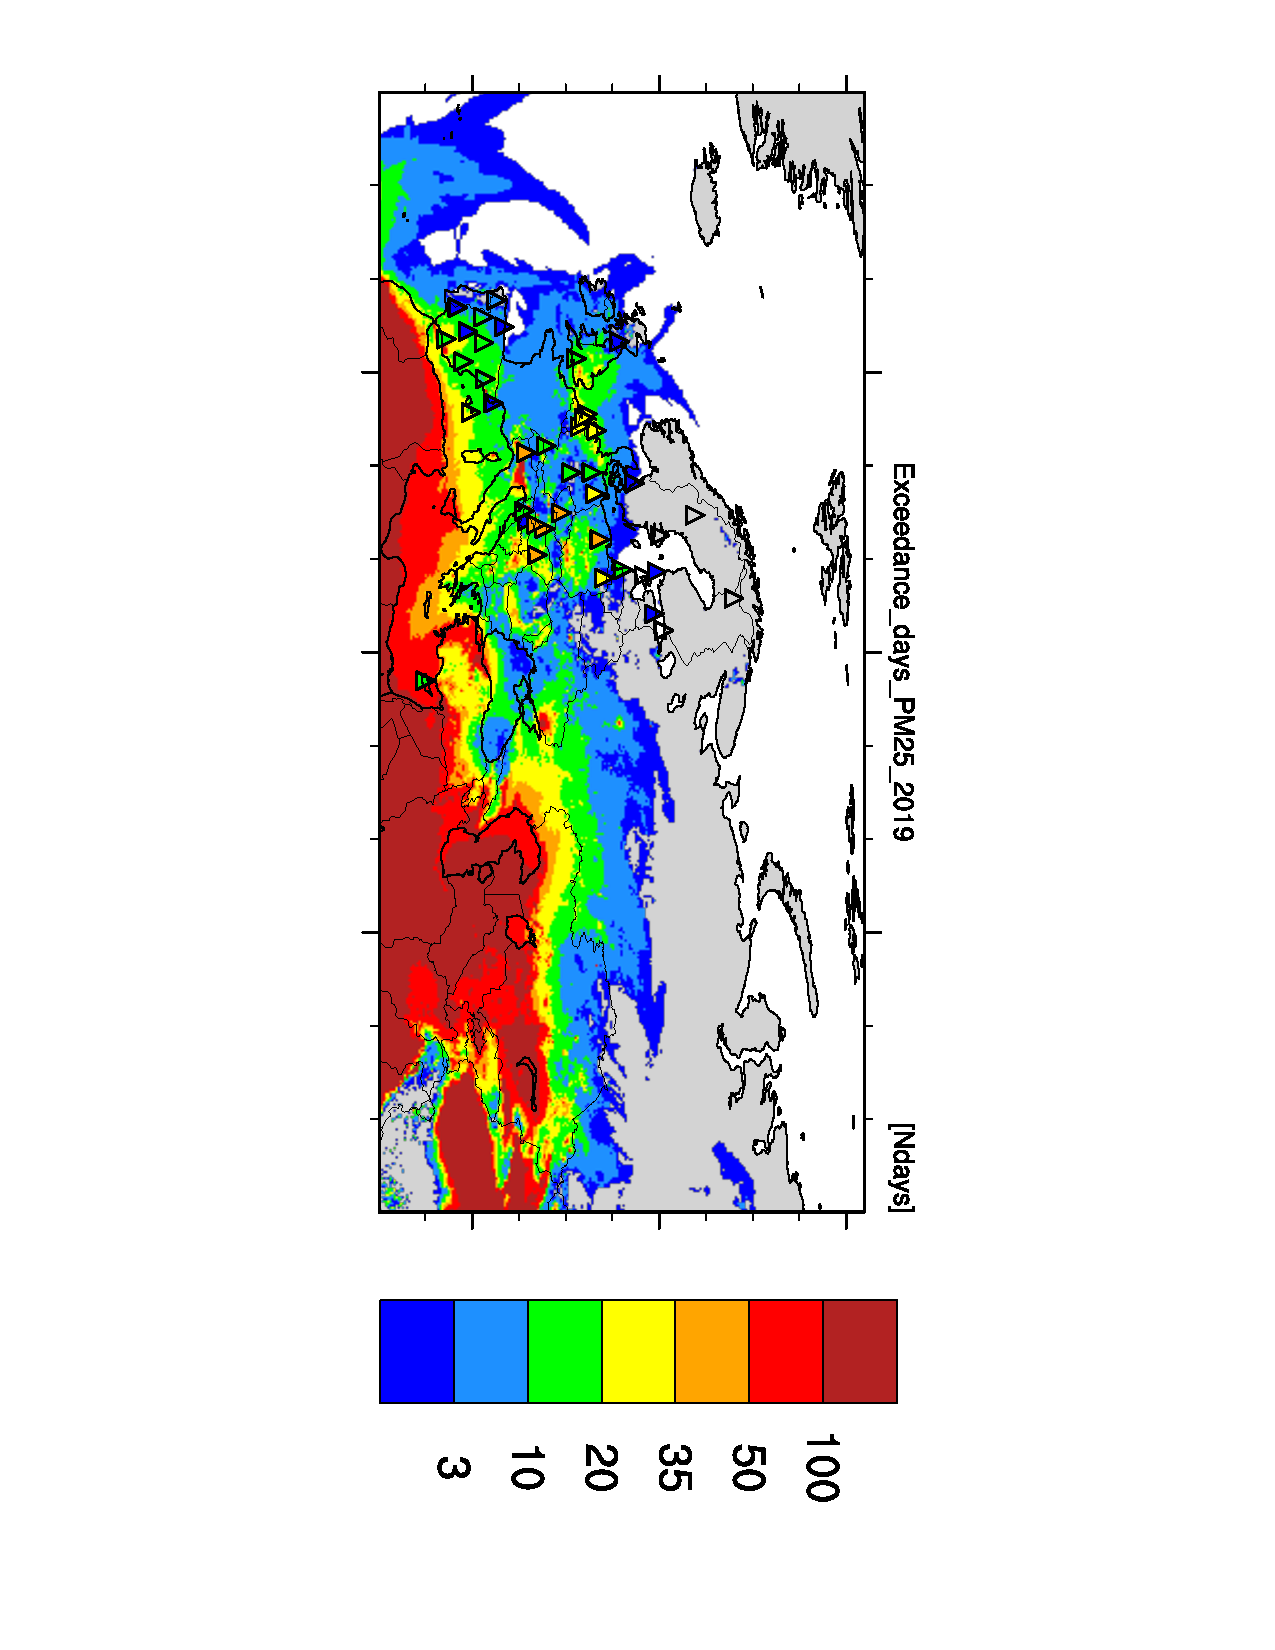
\includegraphics[clip=,angle=90,height=5.9cm,viewport=180 67 440 754]{FIGS_PM/ExcDays_PM25_ModObs_EMEP01_2019.pdf}}
\caption{Calculated (with 0.1\degrees resolution) and observed (triangles) number of days with
  exceedances in 2019: \PM[10] exceeding 50 \ug (upper) and \PM[2.5]
  exceeding 25 \ug (lower panel). \textit{Note: The EU Directive requires no
    more than 35 days with exceedances for \PM[10], whereas WHO
    recommends no more than 3 days with exceedances for \PM[10] and
    \PM[2.5] per calendar year. }}
\label{fig:PMexceed}
\end{figure}


The maps in Figure~\ref{fig:PMexceed} show the number of days with
exceedances of 50 \ug for \PM[10] and 25 \ug for \PM[2.5] in 2019:
modelled values as colour contours and observed values as triangles.

Out of the 67 sites with daily or hourly \PM[10] measurements with data
coverage above 75\%, exceedance days were observed at 31 sites. No
violations of the \PM[10] EU limit value (more than 35 exceedance
days) were observed. Still, 12 sites had more than 3 exceedance days
(according to WHO AQG recommendations). The highest numbers of days
with observed exceedances of \PM[10] were 7 at DE0001 and 6 at LV0010 and RS0005.

\PM[2.5] concentrations exceeded the WHO AQG value at 21 out of 51
stations in 2019. Among those, at 21 sites the number of exceedance
days were more than 3 (the recommended limit according to WHO AQG). 
The highest number of exceedance days was 40, observed at HU0002 and IT0004, followed by 30, 26 and 24 exceedance days at DE0044, PL0005 and AT0002, respectively.

The modelled number of exceedance days in 2019 shows in general a good correspondence with the observations, with somewhat better agreement for \PM[10] than for \PM[2.5]. For \PM[10], the model happens to underestimate the occurrence of exceedances of the EU limit value of 50 \ug for some central European sites, for instance for AT0002 and the Dutch sites NL0009 and NL0010 (no modelled exceedance days versus 5 observed), and in the Baltic for LV0010 (0 exceedance day vs. 6 observed). On the other hand, the model tends to overestimate the number of exceedance days at some Mediterranean sites, influenced by Saharan dust, e.g. at the Cypriot site CY0002 (21 vs. 4 observed) and several Spanish sites (in particular ES0007 with 21 vs. 2 observed). Most of the exceedances registered at the central European sites occurred during the winter (mainly caused by residential combustion) and in the spring (often due to agricultural emissions), while little exceedances occurred in the autumn 2019, which was rather wet. By contrast, at the Mediterranean sites the exceedances were more frequent during summer.

For \PM[2.5], the model reproduces number of exceedance days at IT0004 (40), with most of then (61 \%) coinciding with the observed ones. However, it calculates 12 exceedance days versus 40 observed at HU0002, only 3 versus 30 observed at DE0044, and no exceedance days versus 26 observed at PL0005. At the Dutch sites, the model slightly underestimates observed \PM[2.5] exceedance days at NL0009 and NL0010, but overestimates those at NL0091 and NL0644 (same as for 2018 reported last year). Similar to \PM[10], the model calculates a larger number of exceedance days for \PM[2.5] compared with observations at CY0002 (47 vs 3 observed) and several Spanish sites, which is related to the uncertainties in windblown dust modelling. The seasonality of \PM[2.5] exceedances is similar to that of \PM[10], with most exceedance days at the Mediterranean sites in summer and at the other sites in winter, spring and autumn. The only difference is that the largest number of \PM[2.5] exceedances at three of four German sites occurred in spring, while much fewer occurred during the cold seasons.


\textcolor{blue}{Much rain in November-December combined with the mild winter temperatures, resulted in the absence of major PM episodes in 2019 typical for Europe in winters.} 

%\clearpage
\subsection{Deposition of sulphur and nitrogen} %Hilde to rewrite. Anna to update figures. Done, some final checks on numbers are necessary
\label{subs:dep}


\begin{figure}[H]
  \centering
  \subfigure[oxidized S] {\includegraphics*[viewport=187 62 415 750,clip,angle=90,scale=0.60]{FIGS_STATUS/Mean_in_2019_DEP_SOX_EMEP01.pdf}}
  \subfigure[oxidized N] {\includegraphics*[viewport=187 62 415 750,clip,angle=90,scale=0.60]{FIGS_STATUS/Mean_in_2019_DEP_OXN_EMEP01.pdf}}
  \subfigure[Reduced N] {\includegraphics*[viewport=187 62 415 750,clip,angle=90,scale=0.60]{FIGS_STATUS/Mean_in_2019_DEP_RDN_EMEP01.pdf}} 
 \caption{Deposition of sulphur and nitrogen [mg(S)m$^{-2}$, mg(N)m$^{-2}$] in 2019.}
\label{deps}
\end{figure}

Modelled total depositions of sulphur and oxidised and reduced nitrogen are presented in Figure \ref{deps}.
For sulphur, many hot spots are found in the south-eastern part of the domain. In addition, volcanic emissions of SO$_2$ lead to high depositions in and around Sicily.

Oxidised nitrogen depositions are highest in northern Germany, the Netherlands, Belgium, Poland and northern Italy. These countries also have high depositions of reduced nitrogen, as do parts of the United Kingdom, France and Belgium in western Europe, and Turkey, Georgia, Armenia, Azerbaijan, Kyrgyzstan, Uzbekistan and Tajikistan in the east. 

In Figure \ref{wdeps} wet depositions of nitrogen and sulphur compounds are compared to measurements at EMEP sites for 2019. Overall, the bias of the model with respect to measurements is around 
-32\% to +19\% (Appendix~\ref{ch:appx_modeleval}), but higher for individual sites. A more detailed comparison between model and measurements for the year 2019 can be found at \url{https://aeroval.met.no/evaluation.php?project=emep&exp_name=2021-reporting}.

\begin{figure}[H]
  \centering
  \subfigure[oxidized S] {\includegraphics*[viewport=187 62 415 750,clip,angle=90,scale=0.60]{FIGS_STATUS/so4wdep_2019_ModObs_EMEP01.pdf}}
  \subfigure[oxidized N] {\includegraphics*[viewport=187 62 415 750,clip,angle=90,scale=0.60]{FIGS_STATUS/no3wdep_2019_ModObs_EMEP01.pdf}}
   \subfigure[Reduced N] {\includegraphics*[viewport=187 62 415 750,clip,angle=90,scale=0.60]{FIGS_STATUS/nhxwdep_2019_ModObs_EMEP01.pdf}} 
 \caption{Modelled wet deposition of sulphur and nitrogen [mg(S)m$^{-2}$, mg(N)m$^{-2}$] in 2019, with EMEP observations on top (marked by triangles).}
\label{wdeps}
\end{figure}

\clearpage
\bibliographystyle{copernicus}         % change bibliography-name after each
\renewcommand\bibname{References}      % bibliographystyle command!
\addcontentsline{toc}{section}{References}
\bibliography{Refs2021}
